%%%%%%%%%%%%%%%%%%%%%%%%%%%%%%%%%%%%%%%%%%%%%%%%%%
%%%%%%%%%%%%%%%%%%%%%%%%%%%%%%%%%%%%%%%%%%%%%%%%%%
%%
%% Based one the "beamer-greek-two" template provided 
%% by the Laboratory of Computational Mathematics, 
%% Mathematical Software and Digital Typography, 
%% Department of Mathematics, University of the Aegean
%% (http://myria.math.aegean.gr/labs/dt/)
%%
%% Adapted by John Liaperdos, October-November 2014
%% (ioannis.liaperdos@gmail.com)
%%
%% Last update: 22/06/2017 (English Support)
%%
%%%%%%%%%%%%%%%%%%%%%%%%%%%%%%%%%%%%%%%%%%%%%%%%%%
%%%%%%%%%%%%%%%%%%%%%%%%%%%%%%%%%%%%%%%%%%%%%%%%%%
%%
\PassOptionsToPackage{unicode}{hyperref}
\PassOptionsToPackage{naturalnames}{hyperref}
%\documentclass{beamer} 
\documentclass[aspectratio=169, professionalfonts]{beamer} 

%\usepackage{babel}
%\usepackage[utf8]{inputenc}


%%% FONT SELECTION %%%%%%%%%%%%%%%%%
%%% we choose a sans font %%%%%%%%%%
\usepackage{kmath,kerkis} 
%\usepackage[default]{gfsneohellenic} 

% Use Times NR as font
%\usepackage{newtxtext,newtxmath}
%%%%%%%%%%%%%%%%%%%%%%%%%%%%%%%%%%%%

\usepackage{color}
\usepackage{amsmath}
\usepackage{amssymb}

\usepackage{pgfgantt}
\usepackage{adjustbox}

%\usepackage{media9}
\usepackage{multimedia}

\usepackage{hyperref}
\hypersetup{
    colorlinks=true,
    linkcolor=black,
    filecolor=hslu_pink,      
    urlcolor=hslu_pink,
}

% Have subfigures and captions
\usepackage{subcaption}
\usepackage{caption}

% Tikz to crate diagrams, thanks to: https://github.com/mvoelk/nn_graphics
% Start of tikz settings
\usepackage{tikz}
\usetikzlibrary{positioning,arrows.meta}
\usetikzlibrary{matrix, chains, positioning, decorations.pathreplacing, arrows}
\usetikzlibrary{shapes,arrows,positioning,calc,chains,scopes}

\usepackage{ifthen}
\usepackage{pgfplots}
\pgfplotsset{compat=1.16}
\pgfplotsset{every axis/.append style={tick label style={/pgf/number format/fixed},font=\scriptsize,ylabel near ticks,xlabel near ticks,grid=major}}

\usepackage{amsmath}
\DeclareMathOperator{\sigm}{sigm}
\newcommand{\diff}{\mathop{}\!\mathrm{d}}

% colors
\definecolor{snowymint}{HTML}{E3F8D1}
\definecolor{wepeep}{HTML}{FAD2D2}
\definecolor{portafino}{HTML}{F5EE9D}
\definecolor{plum}{HTML}{DCACEF}
\definecolor{sail}{HTML}{A3CEEE}
\definecolor{highland}{HTML}{6D885A}

\tikzstyle{signal}=[arrows={-latex},draw=black,line width=1pt,rounded corners=4pt]

% RNN
\tikzstyle{block}=[draw=black,line width=1.0pt]
\tikzstyle{cell}=[style=block,draw=highland,fill=snowymint,
    rounded corners]
\tikzstyle{celllayer}=[style=block,draw,fill=portafino,
    inner sep=1pt,outer sep=0,
    minimum width=28pt, minimum height=14pt]
\tikzstyle{pointwise}=[style=block,ellipse,fill=wepeep,
    inner sep=1pt,outer sep=0, minimum size=12pt]

\def\iolen{24pt}
\def\intergape{2pt}

% MLP and CNN
\tikzstyle{netnode}=[circle, inner sep=0pt, text width=22pt, align=center, line width=1.0pt]
\tikzstyle{inputnode}=[netnode, fill=sail, draw=black]
\tikzstyle{hiddennode}=[netnode, fill=snowymint, draw=black]
\tikzstyle{infonode}=[netnode, fill=portafino, draw=black, inner sep=6pt, font=\Large]
\tikzstyle{outputnode}=[netnode, fill=plum, draw=black]

% Architecture
\def\layerwidth{120pt}
\def\layerheight{30pt}

\tikzstyle{layer}=[style=block, draw, fill=black!20!white,
    inner sep=5pt,outer sep=0pt, font=\footnotesize,
    text centered, align=center,
    minimum width=\layerwidth, minimum height=\layerheight]

\tikzstyle{fc}=[style=layer, fill=blue!30!white]
\tikzstyle{conv}=[style=layer, fill=green!30!white]
\tikzstyle{activation}=[style=layer, fill=orange!30!white]
\tikzstyle{pool}=[style=layer, fill=red!30!white]
\tikzstyle{bn}=[style=layer, fill=cyan!30!white]
\tikzstyle{recurrent}=[style=layer, fill=purple!30!white]
\tikzstyle{softmax}=[style=layer, fill=yellow!30!white]
\tikzstyle{point}=[]
\tikzstyle{branch}=[coordinate]

\def\vlayerwidth{30pt}
\def\vlayerheight{3pt}
\def\vblockheight{28pt}

\tikzstyle{vlayer}=[minimum width=\vlayerwidth, minimum height=\vlayerheight]
\tikzstyle{vblock}=[minimum width=\vlayerwidth, minimum height=\vblockheight, text width=1cm, align=center]


% Precision, Recall
\colorlet{fn}{gray!90!green!30!white}
\colorlet{tp}{green!40!white}
\colorlet{fp}{red!40!white}
\colorlet{tn}{gray!90!red!20!white}

\usepackage{ifthen}
\usepackage{pgfplots}
\pgfplotsset{compat=1.16}
\pgfplotsset{every axis/.append style={tick label style={/pgf/number format/fixed},font=\scriptsize,ylabel near ticks,xlabel near ticks,grid=major}}

% equations with term definitions, credit to tex.stackexchange.com/questions/95838/how-to-write-a-perfect-equation-parameters-description
\newenvironment{conditions}
  {\par\vspace{\abovedisplayskip}\noindent\begin{tabular}{>{$}l<{$} @{${}={}$} l}}
  {\end{tabular}\par\vspace{\belowdisplayskip}}
  
\newenvironment{conditions*}
  {\par\vspace{\abovedisplayskip}\noindent
   \tabularx{\columnwidth}{>{$}l<{$} @{${}={}$} >{\raggedright\arraybackslash}X}}
  {\endtabularx\par\vspace{\belowdisplayskip}}

\usepackage{epstopdf}
\usepackage{graphicx}
\graphicspath{{./images/}}

% to make beautiful tables
\usepackage{booktabs}

% appendix for beamer
\usepackage{appendixnumberbeamer}

% notes on beamer template
\usepackage{pgfpages}
\setbeameroption{show notes}
\setbeameroption{show notes on second screen=right}

%%
% load TEI-Pel - specific layout
\usepackage{HSLU_Thesis_Beamer_Layout}
\setTeipelLayout{}% options: "draft" -> Watermark

\setcounter{tocdepth}{1}
%\beamertemplatenavigationsymbolsempty
\setbeamertemplate{headline}{}

%%%%%%%%%%%%%%%%%%%%%%%%%%%%%%%%%%%%%%%%%%%%%%%%%%%%%%%%%%%%
% Thesis Info %%%%%%%%%%%%%%%%%%%%%%%%%%%%%%%%%%%%%%%%%%%%%%
%%%%%%%%%%%%%%%%%%%%%%%%%%%%%%%%%%%%%%%%%%%%%%%%%%%%%%%%%%%%
	% title
		\title[Deep Embedded Music]{Presentation\\ Deep Embedded Music}	
	% author 
		\author[F. Gröger]{Fabian Gröger}
	% supervisor	
		\supervisor{Supervisor}{Daniel Pfäffli, HSLU}{Expert}{Dr. Jeremy Callner, APG/SGA}
	% date
		\presentationDate{\today}
%%%%%%%%%%%%%%%%

\begin{document}

% typeset front slides
	\typesetFrontSlides

%%%%%%%%%%%%%%%%
% Start of Slides:

%%%%
\section{Project overview}

%%

\begin{frame}{Project overview}
	\framesubtitle{unsupervised embedding space for audio}
	\begin{itemize}
		\item create an \textbf{embedding space for audio}, using \textbf{unsupervised machine learning}
        \item adapt \textbf{Tile2Vec}, an image embedding algorithm, to audio
        \item evaluate the \textbf{performance on the DCASE 2018 task 5 dataset}
        \item \textbf{train a simple classifier} on the embeddings
        \item the resulting embedding algorithm should be \textbf{applied exploratively to music}
	\end{itemize}
	
	\note{
	    \begin{itemize}
	        \item \textbf{1:15}
	    \end{itemize}
	}
\end{frame}

%%%%
\section{Project management}

%%

\begin{frame}{Project management:}
    \begin{figure}
    \centering
         \resizebox{11cm}{!}{\begin{ganttchart}[%Specs
         x unit = 1.05cm,  %<---------------------- New x unit 
         y unit title=0.4cm,
         y unit chart=0.5cm,
         vgrid, hgrid,
         title height=1,
         title label font=\bfseries\footnotesize,
         bar/.append style={fill=blue!50},
         group/.append style={draw=black, fill=orange!40!white},
         milestone/.append style={draw=black, fill=red!40!white, xscale=0.55}, % 0.5/0.9 ≈ 0.5555
         milestone progress label node/.append style={right=0.2},
         bar incomplete/.append style={fill=none},
         group incomplete/.append style={draw=black,fill=none},
         bar height=0.7,
         group right shift=0,
         group top shift=0.5,
         group height=.3,
         group peaks width={0.2},
         inline]{1}{15}
        %labels
    
        %\gantttitle{bachelor thesis - deep embedded music}{18}\\
        \gantttitle[]{2020}{15} \\                
        \gantttitle{Feb}{2}
        \gantttitle{Mar}{4}
        \gantttitle{Apr}{4}
        \gantttitle{May}{4}
        \gantttitle{Jun}{1}\\
        
        % 1. Phase: Research
        \ganttgroup[inline=false]{Research}{1}{4}\\ 
        \ganttbar[progress=100,inline=false]{Dataset}{1}{1}\\
        \ganttbar[progress=100,inline=false]{Audio processing}{1}{1}\\
        \ganttbar[progress=100,inline=false]{Triplet loss}{2}{2}\\
        \ganttbar[progress=100,inline=false]{Tile2Vec}{3}{3}\\
        \ganttbar[progress=100,inline=false]{Evaluate research}{4}{4}\\
        \ganttmilestone[inline=false]{Research finished}{4} \\ % M1
        
        % 2. Phase: Realization
        \ganttgroup[inline=false]{Realisation}{5}{8} \\
        \ganttbar[progress=100,inline=false]{Project setup}{5}{5} \\
        \ganttbar[progress=100,inline=false]{Input pipeline}{5}{5} \\
        \ganttbar[progress=100,inline=false]{Default model architectures}{6}{6} \\
        \ganttbar[progress=100,inline=false]{Evaluation workflow}{6}{6} \\
        \ganttbar[progress=100,inline=false]{Unit tests}{6}{6} \\
        \ganttmilestone[inline=false]{Project Setup finished}{6} \\ % M2
        \ganttbar[progress=100,inline=false]{Tile2Vec implementation}{7}{7} \\
        \ganttbar[progress=100,inline=false]{Architecture for experiments}{8}{8} \\
        \ganttmilestone[inline=false]{Realisation finished}{8} \\ % M3
        
        \ganttmilestone[inline=false]{Interim presentation}{9} \\ % M3
        
        % 3. Phase: Experiments
        \ganttgroup[inline=false]{Experiments}{9}{12} \\
        \ganttbar[progress=100,inline=false]{Conduct experiments}{9}{9} \\
        \ganttbar[progress=100,inline=false]{Validate embeddings}{10}{11} \\
        \ganttmilestone[inline=false]{Experiments finished}{11} \\ % M4
        \ganttbar[progress=100,inline=false]{Visualise embeddings}{12}{12} \\
        
        % Buffer
        \ganttgroup[inline=false]{Buffer}{13}{13} \\
        
        % 4. Phase: Documentation
        \ganttgroup[inline=false]{Finalise documentation}{14}{15} \\
        \ganttbar[progress=100,inline=false]{Create pitch video and web abstract}{14}{14} \\
        \ganttbar[progress=100,inline=false]{Finalise documentation}{14}{15} \\
        \ganttbar[progress=100,inline=false]{Proofread documentation}{15}{15} \\
        \ganttmilestone[inline=false]{Thesis submission}{15}
    \end{ganttchart}}
    %\caption{Project plan}
    \label{fig:Project-Plan}
    \end{figure}
    
    \note{
        \begin{itemize}
            \item \textbf{1:45}
            \item as you may still remember, I have chosen an iterative waterfall procedure model
            \item and as you can see I was able to deliver all of the planned work packages and therefore fulfill my project plan
        \end{itemize}
    }
\end{frame}

%%%%
\section{Related work}

%%
\subsection{Audio feature representations}

\begin{frame}{Related work}
    \framesubtitle{log Mel spectrogram and MFCCs}
    \begin{columns}[T]

        \column{0.6\textwidth}
            \begin{itemize}
        		\item Mel frequency cepstral coefficients (MFCCs) and log Mel spectrograms \textbf{focus on the audio signal} and \textbf{discard information such as background noise}
        		\item \textbf{Cepstrum} is the information on the rate of change in spectral bands
                \item MFCC and log Mel spectrograms were designed to \textbf{mimic the human hearing}
        	\end{itemize}
        
        \column{0.4\textwidth}
            \centering
            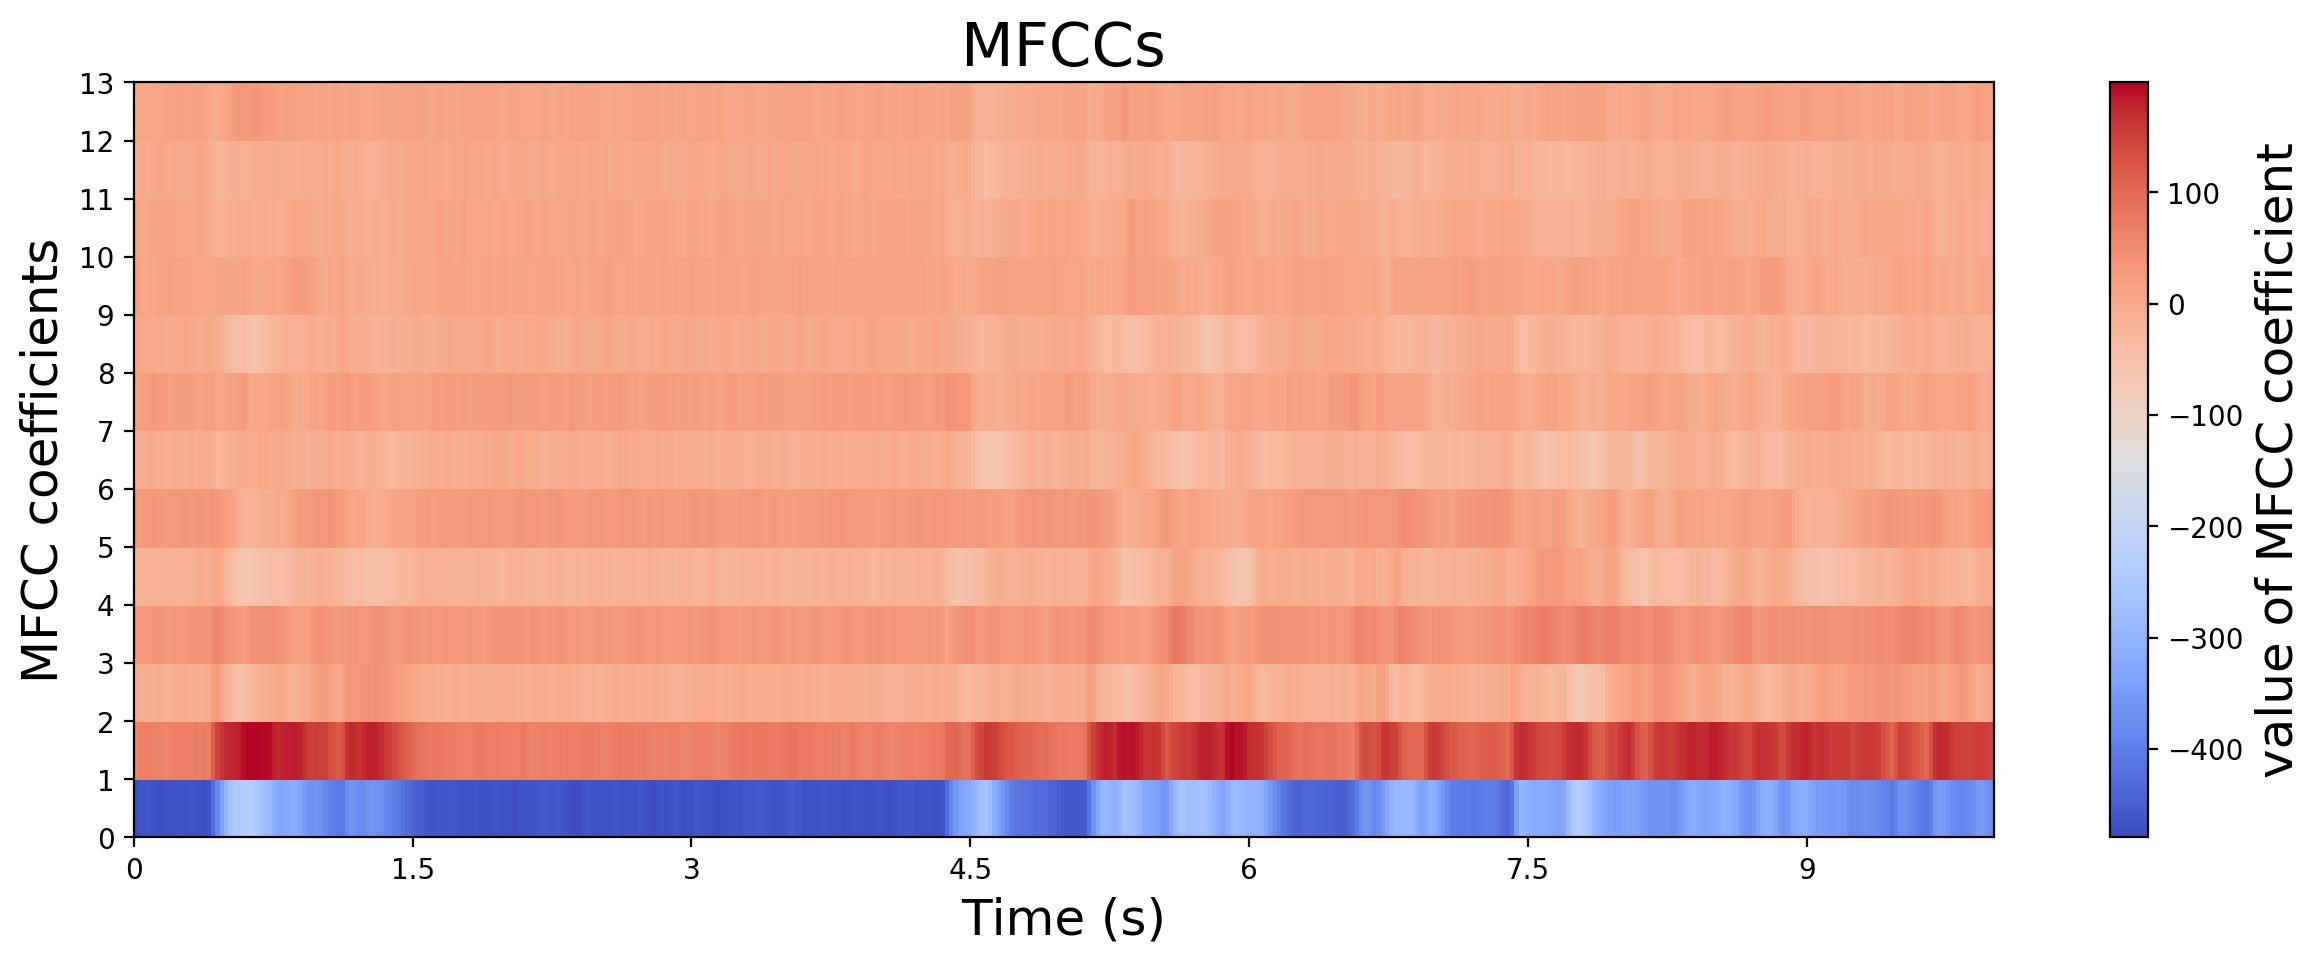
\includegraphics[width=1.0\textwidth,keepaspectratio]{images/mfccs.png}
            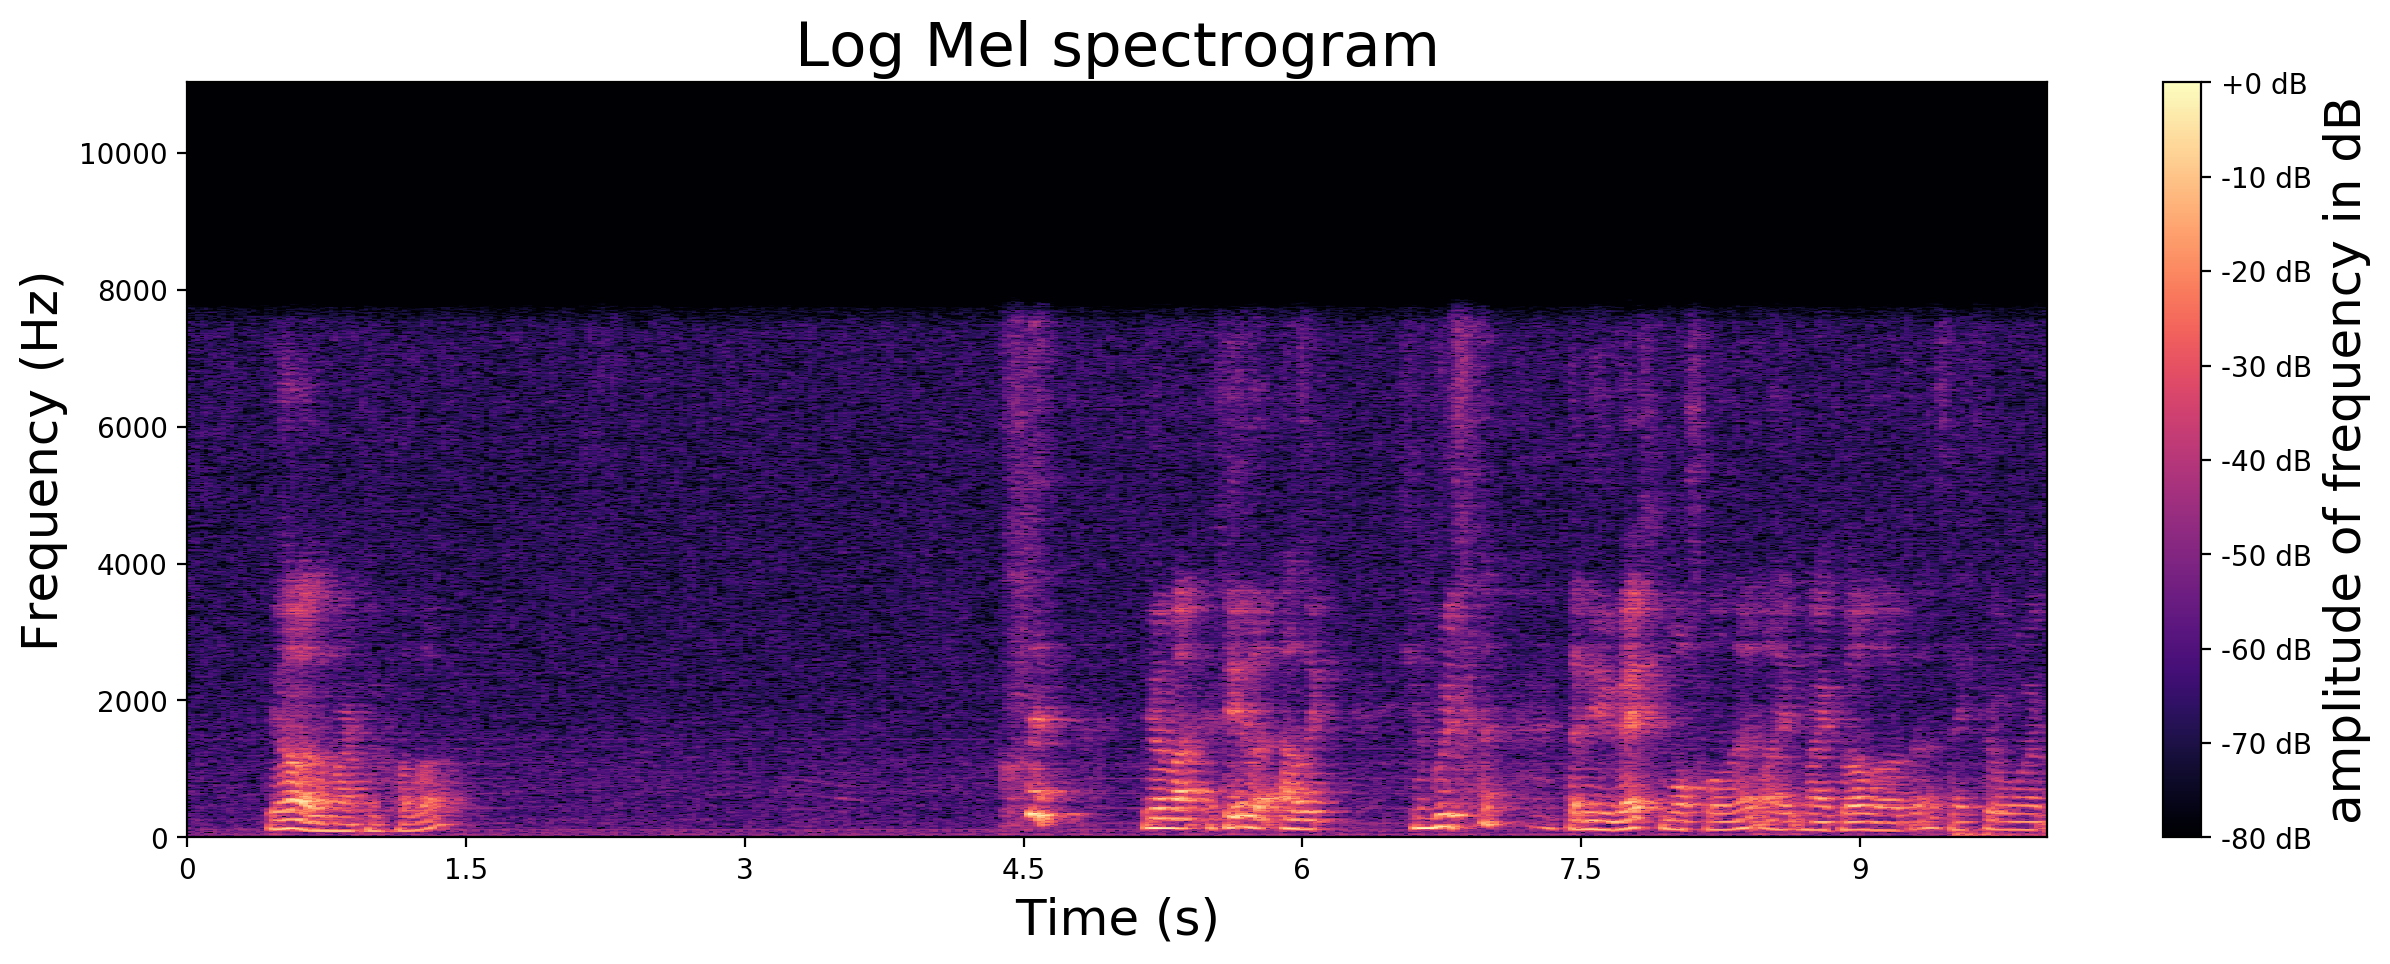
\includegraphics[width=1.0\textwidth,keepaspectratio]{images/log_mel_spectrogram.png}
    \end{columns}
    \\[10pt]
    \begin{figure}[htbp]
	    \small
    	\centering
        \resizebox{14cm}{!}{\begin{tikzpicture}[
            input/.style = {coordinate},
            output/.style = {coordinate},
            block/.style={rectangle, draw, text width=7.3em,
                   text centered, rounded corners, minimum height=3em},
            arrow/.style={-{Stealth[]}}
        ]
            \node [input] (input) {};
            \node [block,right=2.5cm of input] (Frames)  {Break signal into overlapping frames};
            \node [block,right=0.5cm of Frames] (FFT)  {Fast Fourier Transform (FFT)};
            \node [block,right=0.5cm of FFT] (MEL)  {Mel-Scale filter bank};
            \node [block,right=0.5cm of MEL] (LOG) {Log $|\cdot|$};
            \node [block,right=0.5cm of LOG] (DCT) {Discrete Cosine Transform (DCT)};
            \node [output,right=1.5cm of DCT] (output) {};
        
            % Draw edges
            \draw [arrow] (input) -- (Frames) node [above,pos=0.5] {\textbf{continuous audio}} node [below,pos=0.5] {\textbf{signal}};
            \draw [arrow] (Frames) -- (FFT);
            \draw [arrow] (FFT)  --  (MEL);  
            \draw [arrow] (MEL) --  (LOG);  
            \draw [arrow] (LOG) -- node [above=0.5cm] {\textbf{log Mel spectrogram}} (DCT) ;
            \draw [arrow] (DCT) -- node [above,pos=0.5] {\textbf{MFCCs}} (output);
        \end{tikzpicture}}
        %\caption{Steps to calculate MFCC}
        \label{fig:MFCC-Overview}
    \end{figure}
    
    \note{
        \begin{itemize}
            \item \textbf{4:00}
            \item as my thesis focuses on working with audio data, the most important aspect is to represent the audio segments in a more compact format
            \item such a representation is called the feature representation, where I have mainly used two different ones, the MFCCs and log mel spec
            \item 
            \item visual representation of the frequencies in the log Mel scale
        \end{itemize}
    }
	
\end{frame}

\begin{frame}{Related work}
    \framesubtitle{Triplet loss and Tile2Vec}
    \textbf{Triplet loss:}\textsuperscript{\cite{FaceNet}}
	\begin{itemize}
		\item learn distributed \textbf{embeddings} by the \textbf{notion of similarity and dissimilarity} 
		\item triplets consisting of an \textbf{anchor $x_a$}, a \textbf{positive $x_p$} and a \textbf{negative $x_n$} sample
	\end{itemize}
	\begin{equation}
        \centering
        \mathcal{L} = \Bigg [\Big|\Big|f_\theta(x_a) - f_\theta(x_p)\Big|\Big|_2^2 - \Big|\Big|f_\theta(x_a) - f_\theta(x_n)\Big|\Big|_2^2 + \alpha \Bigg]_+
        \label{eq:Triplet-Loss}
    \end{equation}
	\\[10pt]
	\textbf{Tile2Vec:}\textsuperscript{\cite{Tile2Vec}}
	\begin{itemize}
	    \item \textbf{unsupervised triplet loss} by using the \textbf{distributional hypothesis} from natural language (words appearing in similar contexts tend to have similar meanings)
	    \item $x_p$ lies \textbf{within a neighbour radius} from the anchor
	    \item $x_n$ lies \textbf{outside of the neighbour radius}
	    %\item \textbf{$l^2$ - normalisation}, to force embeddings to be within a hypersphere
	\end{itemize}
	
	\note{
	    \begin{itemize}
	        \item \textbf{5:00}
	    \end{itemize}
	}
\end{frame}

\begin{frame}{Dataset used}
    \framesubtitle{DCASE Challenge 2018 - task 5 dataset and music dataset}
    
    \begin{columns}[T]
    
        \column{0.5\textwidth}
        \textbf{noise detection dataset:}\textsuperscript{\cite{DCASE}}
        \begin{itemize}
    		\item derivative of the \textbf{SINS dataset}, a continuous recording of one person living in a vacation home over one week
    		\item \textbf{DCASE: 7 microphone arrays} in the combined living room and kitchen
    		\item continuous recordings were labelled and split into \textbf{audio segments of 10s}
    		\item approximately \textbf{400 hours} of data
    		\item \textbf{winner:} \textbf{88.4\%} macro-averaged F1 score
    	\end{itemize}

        \column{0.5\textwidth}
        \textbf{music dataset:}
        \begin{itemize}
    		\item \textbf{7 different sub genres} with \textbf{30 songs} each
    		\item music genre is considered to be \textbf{electronic dance music}
    		\item songs classified by genre according to \href{https://www.beatport.com/}{beatport.com}
    		\item approximately \textbf{18 hours} of music
    		\item songs \textbf{vary in length}, from 3min to 10min
    		\item single channel \textbf{.mp3 files}
    	\end{itemize}
    \end{columns}
    
    \note{
        \begin{itemize}
            \item \textbf{6:00}
            \item Two different datasets are used within the project, the DCASE dataset which further referred to as the noise detection dataset and the music dataset
        \end{itemize}
    }
\end{frame}

%%%%
\section{Ideas and concepts}

\begin{frame}{Ideas and concepts}
    \framesubtitle{how the project will be realised}
    
    \begin{columns}[T]

        \column{0.5\textwidth}
        \begin{itemize}
    		\item \textbf{data pre-processing:} \\
    		\begin{itemize}
    		    \item DCASE: none \\
    		    \item Music: conversion from {\small \texttt{.mp3}} to {\small \texttt{.wav}}
    		\end{itemize}
    		\item \textbf{feature extraction:} \\
    		\begin{itemize}
    		    \item raw waveform
    		    \item log Mel spectrogram
    		    \item MFCCs
    		\end{itemize}
    		\item \textbf{triplet selection:} songs split into segments, anchor and neighbour belong to the same audio, opposite belongs to a different one (temporal proximity)
    	\end{itemize}
        
        \column{0.5\textwidth}
        \begin{itemize}
            \item \textbf{model:} ResNet
    		\item \textbf{metrics embedding space:}\\
    		\begin{itemize}
    		    \item triplet loss
    		    \item distance to neighbour / opposite
    		    \item distance to clusters (distance matrix)
    		    \item silhouette coefficient
    		\end{itemize}
    		\item \textbf{metrics classifier:} \\
    		\begin{itemize}
    		    \item sparse categorical cross-entropy loss
    		    \item sparse categorical accuracy
    		    \item macro-averaged F1 score
    		\end{itemize}
    	\end{itemize}
    \end{columns}
    
    \note{
        \begin{itemize}
            \item \textbf{8:00}
        \end{itemize}
    }
\end{frame}

%%%%
%\section{Evaluation}

\section{Implementation}

\begin{frame}{Implementation}
    \begin{columns}[T]
        \column{0.5\textwidth}
            \begin{itemize}
        		\item \textbf{Python 3.6.9}
        		\item \textbf{TensorFlow 2.1}
        		\item \textbf{librosa}
        		\item \textbf{multi threaded input pipeline} using \texttt{tf.data.Dataset}
        		\item \textbf{generator} was used, which generates the dataset samples \textbf{on the fly} (including triplet selection and feature extraction)
        		\item GPU \textbf{GTX 1080Ti}, 11 GB RAM
        	\end{itemize}
        
        \column{0.5\textwidth}
            \centering
            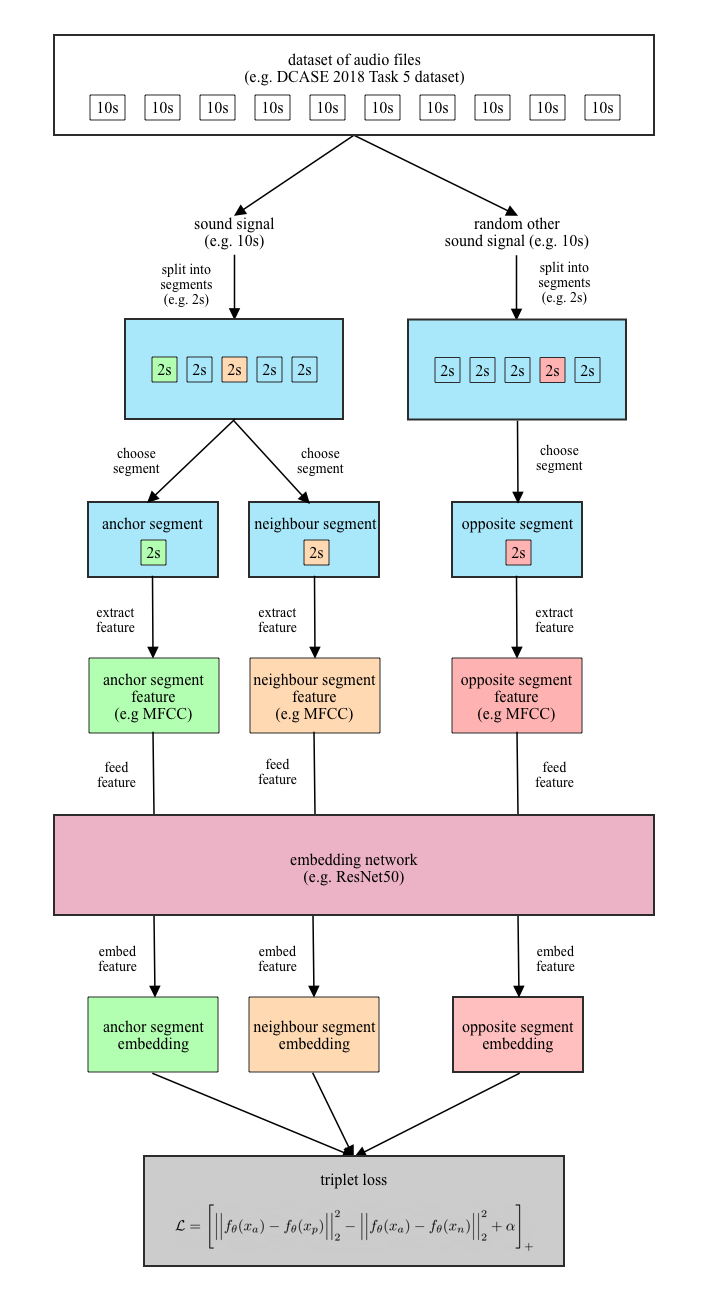
\includegraphics[width=0.5\textwidth,keepaspectratio]{images/Input_Pipeline_Visualisation.png}
    \end{columns}
    
    \note{
        \begin{itemize}
            \item \textbf{9:30}
            \item now coming to the implementation of my thesis
            \item I will not go into much detail, since I want to focus on the results of the thesis rather than the implementation
            \item The reason why a generator function is used, is that the entire dataset can not be loaded into memory, due to the large size of it
            \item advantage of this method is that the pipeline can be adapted fairly quick for other datasets since the only input the pipeline requires is the raw waveform of any audio signal
        \end{itemize}
    }
\end{frame}

\section{Experiments and results}

\begin{frame}{Conducted experiments and findings}
    \framesubtitle{list of all the experiments conducted during the thesis including the most important findings}
    \begin{columns}[T]
        \column{0.5\textwidth}
            \textbf{Experiments conducted:}
            \begin{itemize}
        		\item experiment: margin
        		\item experiment: segment size
        		\item experiment: embedding size
        		\item experiment: regularisation factor
        		\item experiment: feature representation
        		\item experiment: larger embedding size
        	\end{itemize}
        
        \column{0.5\textwidth}
            \textbf{Findings:}
            \begin{itemize}
        		\item \textbf{longer audio segments} resulted in an embedding space with clearer clusters
        		\item the \textbf{log Mel spectrogram} proves to be a better representation for the task than the MFCCs 
        		\item \textbf{triplet loss adaption} with \textbf{zero filtering} provides a great performance increase
        	\end{itemize}
    \end{columns}
    
    \note{
        \begin{itemize}
            \item \textbf{12:00}
            \item now I will first present the experiments, which were conducted during the experiment phase of the thesis and then show you the results of the final models
            \item 6 different experiments were conducted (column left), study doc was written
            \item each one focused on finding an optimal parameter for the embedding space
            \item during the experiment phase important findings were discovered, which will help anyone in the future to successfully train an unsupervised triplet loss for audio
            \item 
            \item the last step of the experiment phase was to train a model until convergence with the optimal hyperparameters found during the experiments for both of the datasets
        \end{itemize}
    }
\end{frame}

\begin{frame}{Model: noise detection dataset}
    \framesubtitle{final model trained on the DCASE 2018 - Task 5 dataset}
    
    \begin{columns}
        \column{0.5\textwidth}
        \centering
        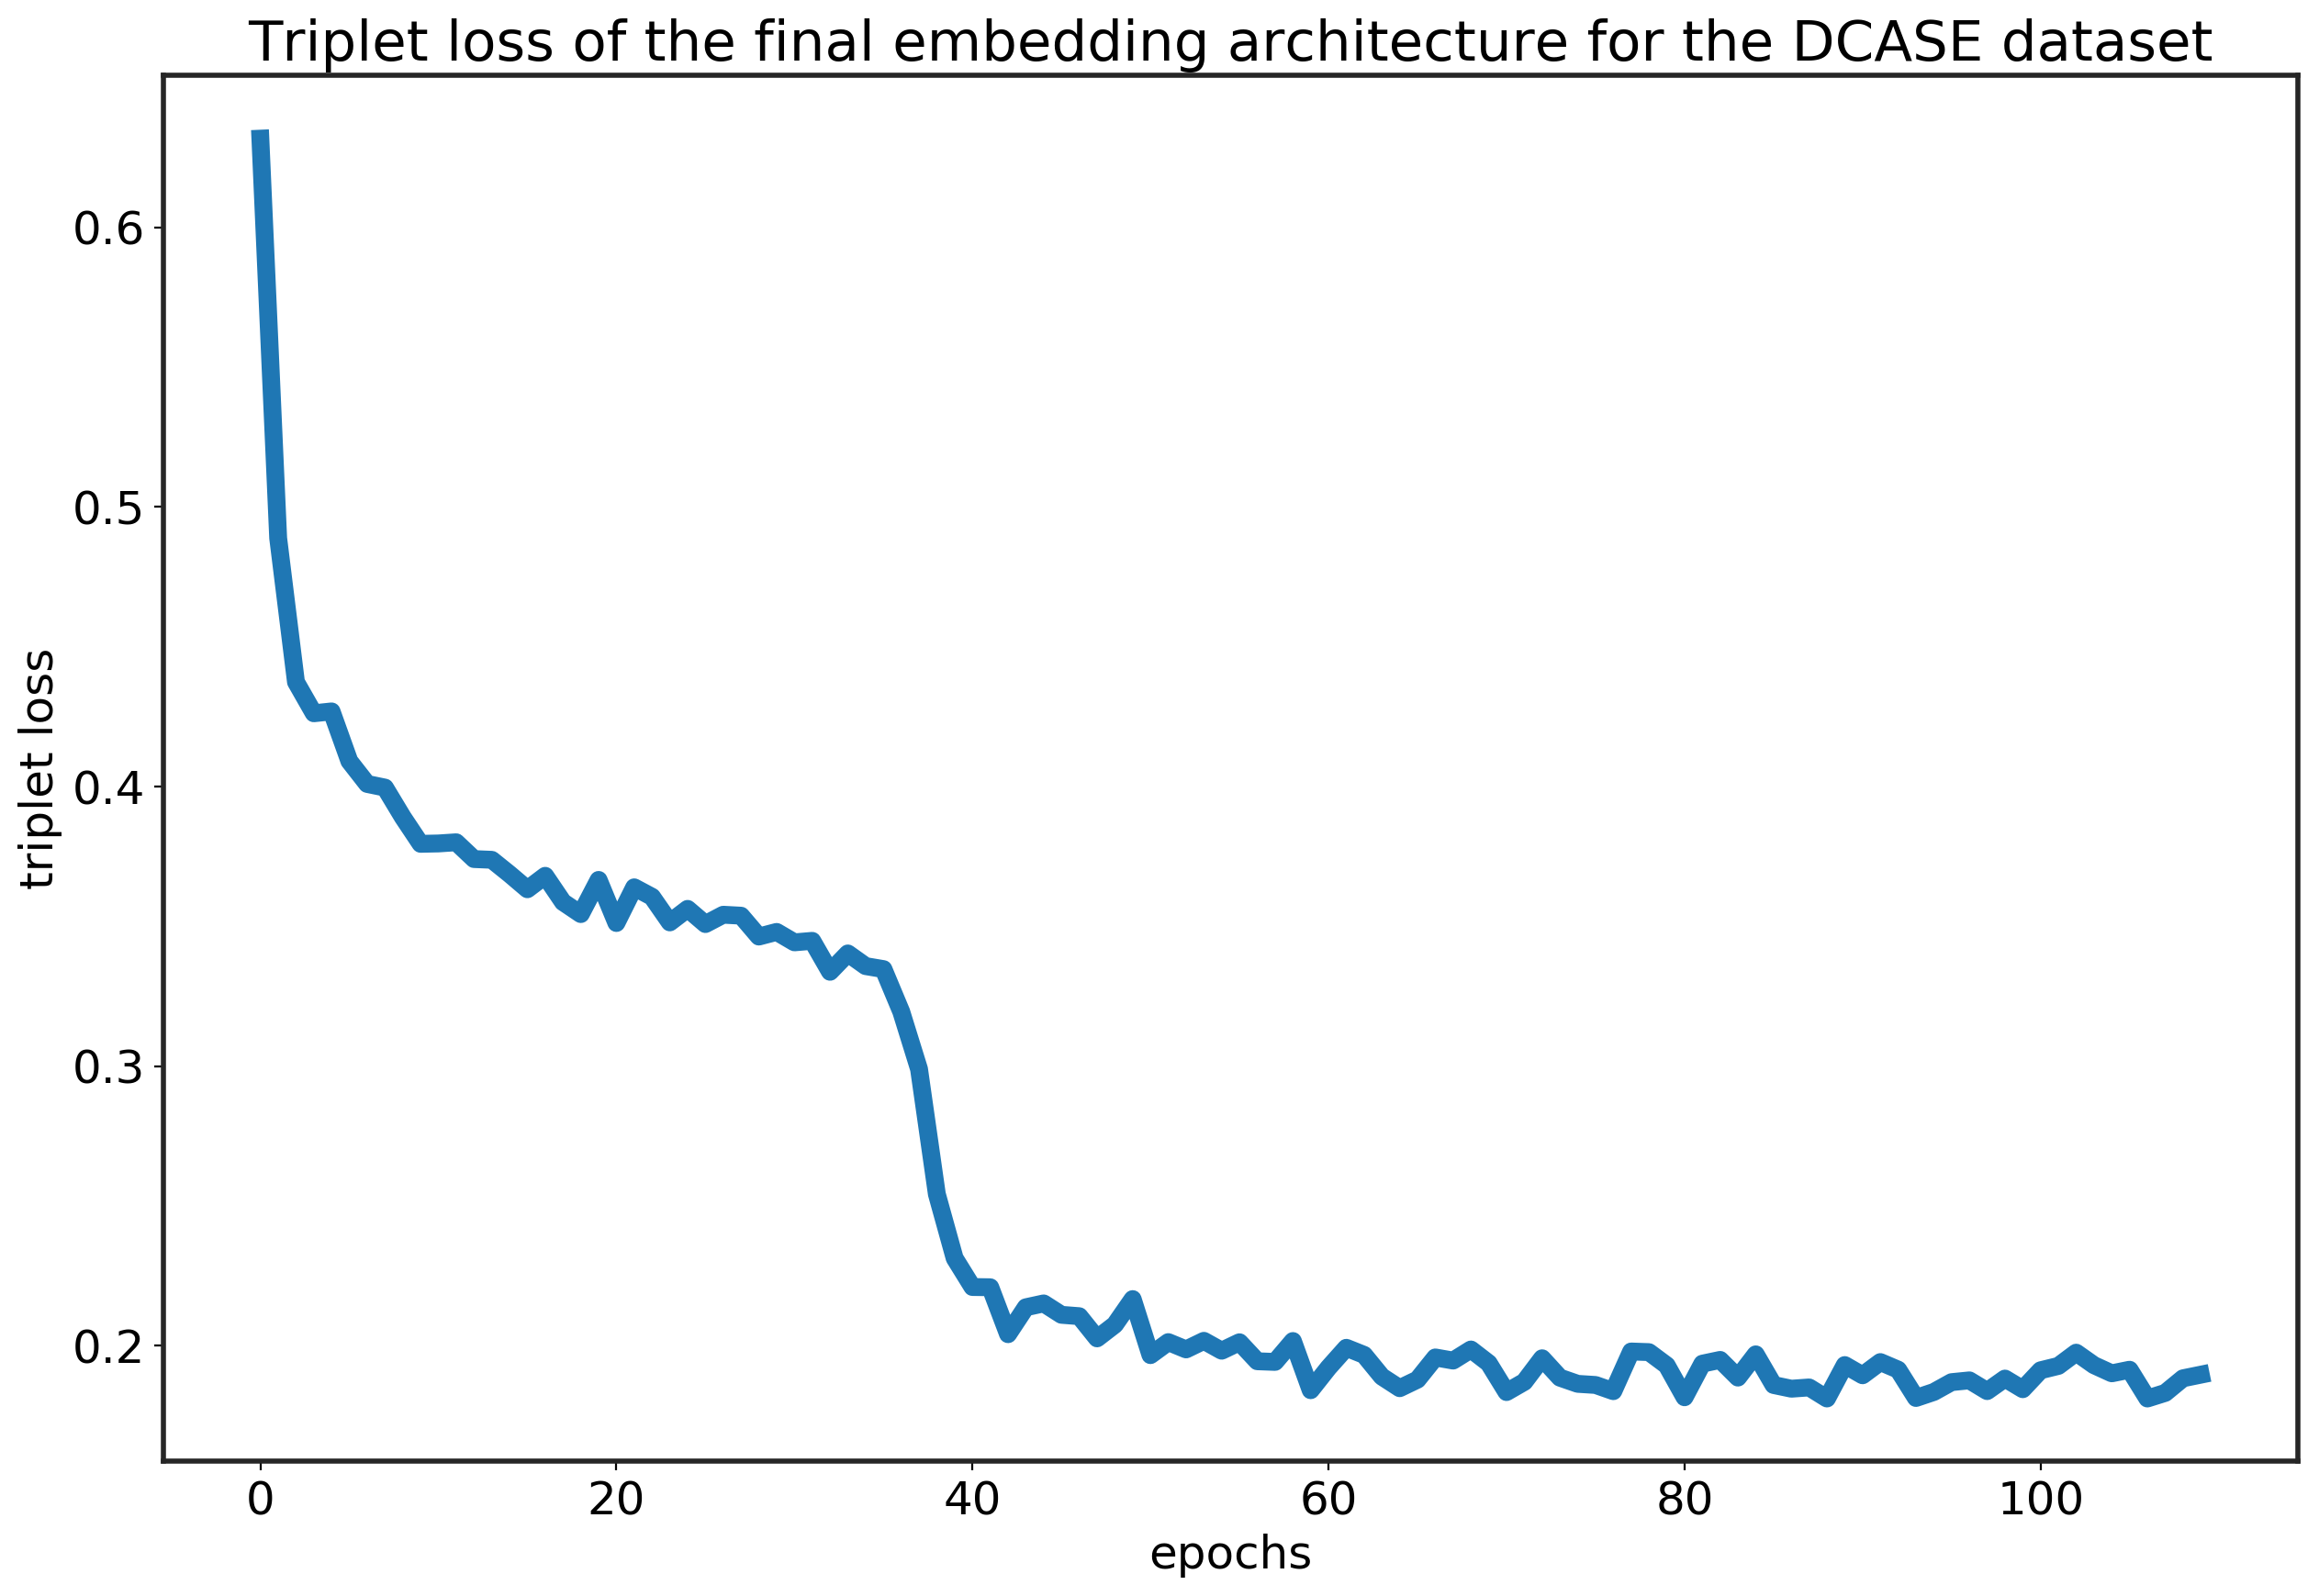
\includegraphics[width=1.0\textwidth,keepaspectratio]{images/Triplet_loss_DCASE_final.png}
    
        \column{0.5\textwidth}
        \begin{table}[htbp]
            \centering
            %\caption{Music genres in the music dataset along with the number of songs}
        	\label{tab:Hyperparameters-DCASE}
        	\tiny
            \begin{tabular}{l|l}
                \toprule
                \textbf{Hyperparameter} & \textbf{value} \\ 
                \midrule[1pt]
                Model & ResNet18 \\ 
                \hline
                Epochs & 110 \\ 
                \hline
                Batch size & 64 \\ 
                \hline
                Optimiser & Adam \\ 
                \hline
                Learning rate & 1e-5 \\
                \hline
                Margin & 1.0 \\
                \hline
                L2 regularisation factor & 0.01 \\
                \hline
                Embedding dimension & 256 \\
                \midrule[1pt]
                \multicolumn{2}{l}{\textit{Audio sample}} \\
                \midrule[1pt]
                Sample rate & 16000 \\ 
                \hline
                Sample segment size & 5s \\
                \hline
                Sample segment range & 5s \\
                \hline
                Convert to mono & True \\
                \midrule[1pt]
                \multicolumn{2}{l}{\textit{Feature representation}} \\
                \midrule[1pt]
                Feature extractor & LogMelExtractor \\ 
                \hline
                Input size & 498 x 128 \\
                \bottomrule
            \end{tabular}
        \end{table}
    \end{columns}
    
    \note{
        \begin{itemize}
            \item \textbf{12:30}
            \item the final model of the noise detection dataset was trained for 110 epochs and the training took around 3 days
            \item the resulting triplet loss value graph is shown in the figure on the left
            \item the used hyperparameters to train the model is shown in the table on the right
        \end{itemize}
    }
\end{frame}

\begin{frame}{Results: noise detection dataset}
    \framesubtitle{final model trained on the DCASE 2018 - Task 5 dataset}
    
    \begin{columns}
        \column{0.5\textwidth}
        \centering
        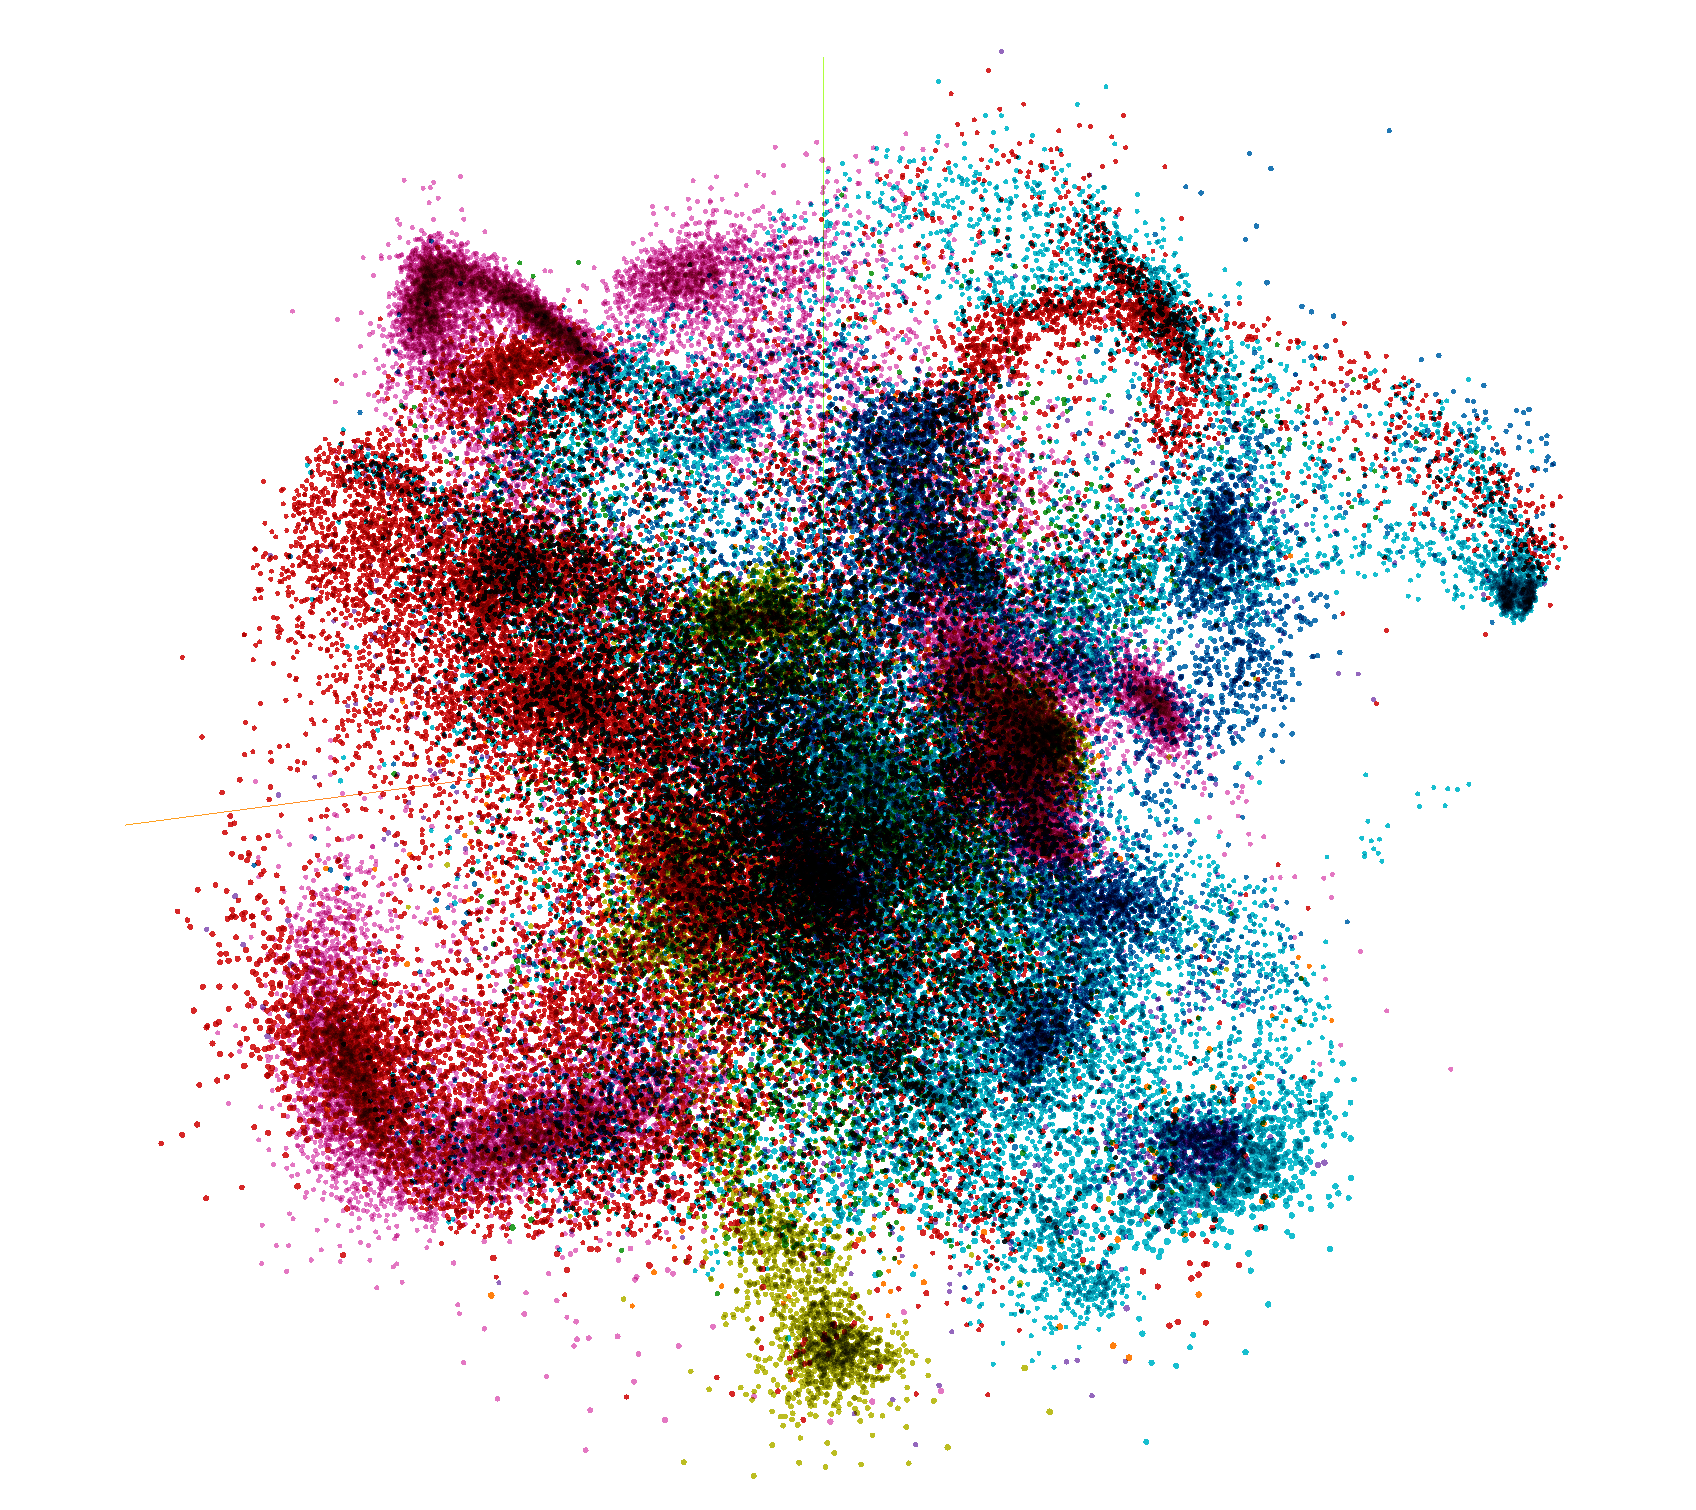
\includegraphics[width=0.7\textwidth,keepaspectratio]{images/embedding_space_dcase.png}
        
        \column{0.5\textwidth}
        \centering
        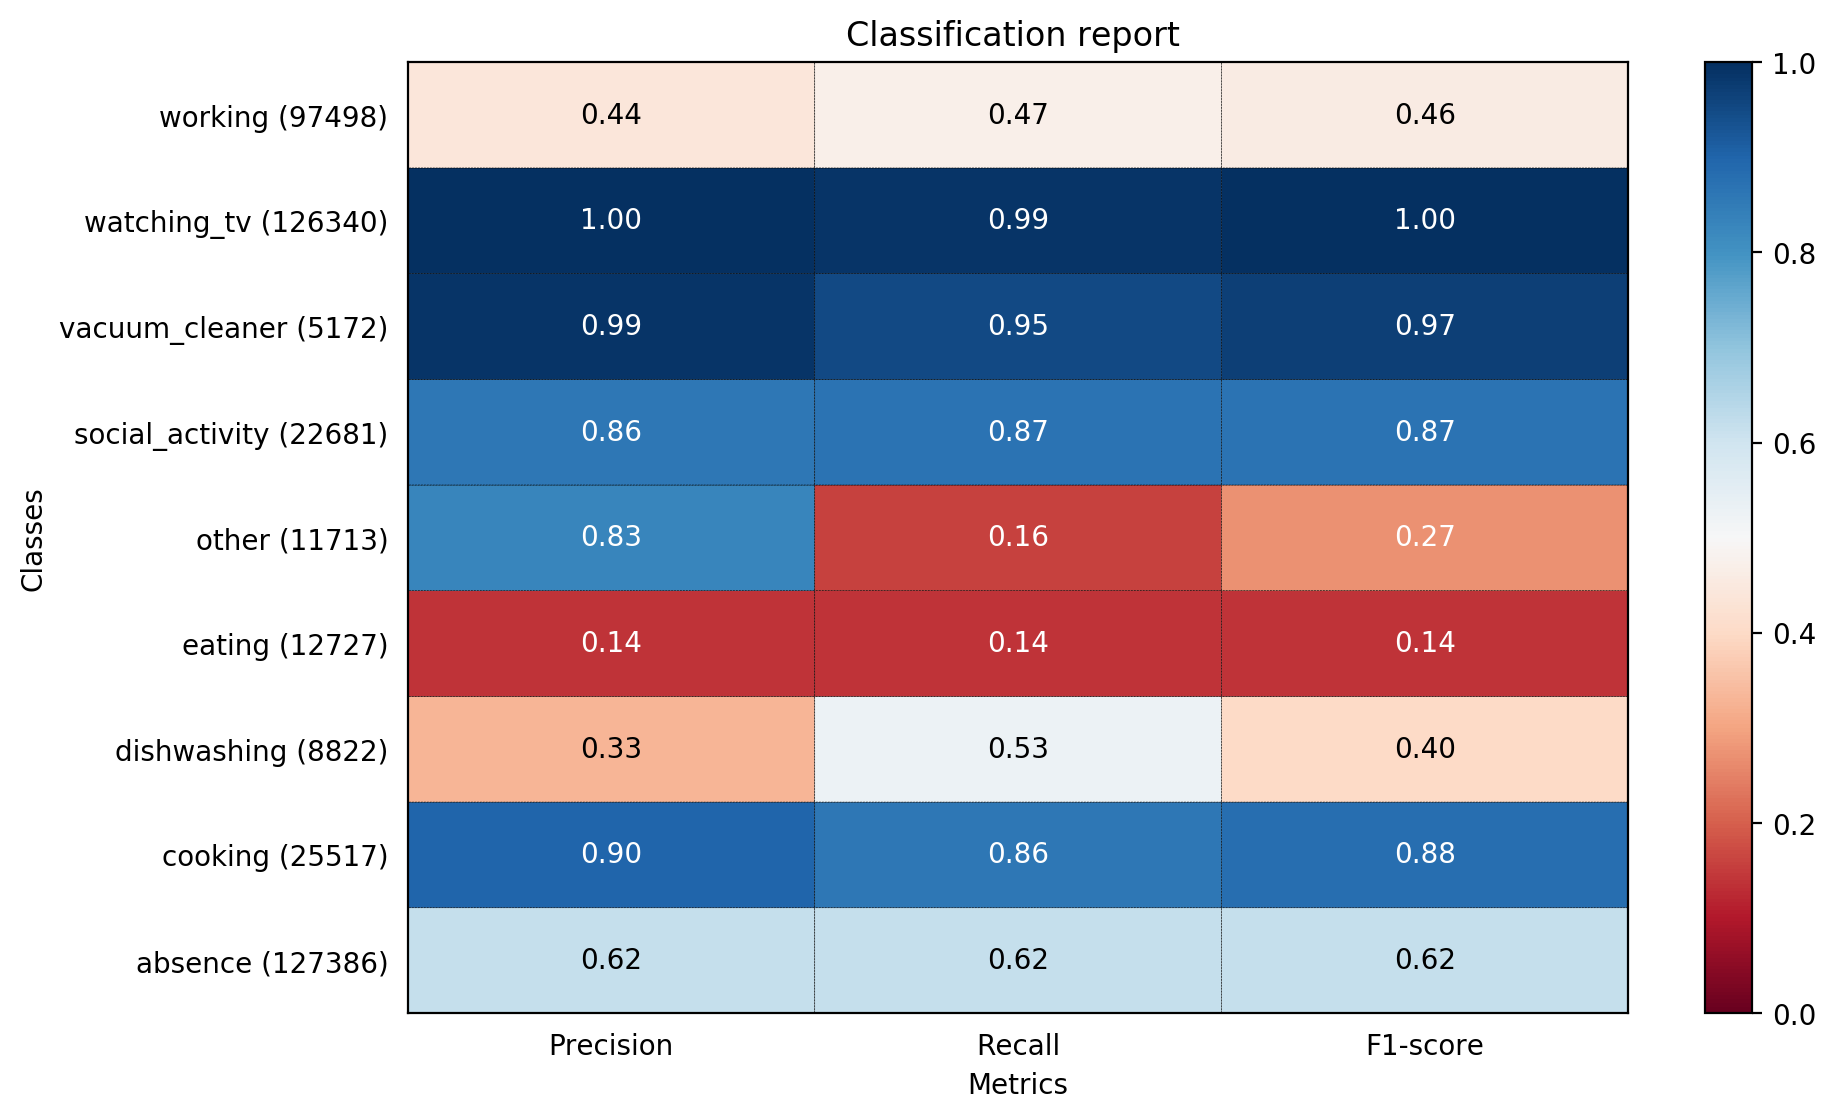
\includegraphics[width=1.0\textwidth,keepaspectratio]{images/DCASE_F1_classification_report.png}
    \end{columns}
    % try to insert audio here
        
    \note{
        \begin{itemize}
            \item \textbf{14:30}
            \item coming to the results of the noise detection dataset
            \item the embedding space was evaluated in two different ways
            \item the first evaluation was to train a simple linear logistic classifier for 40 epochs, using the embedded samples as input in a supervised manner
            \item the results of the classifier are shown in the classification report on the right, where the scores are shown for each one of the classes in the dataset
            \item it reached an macro averaged F1 score of 62\% on the test set from the challenge, which is approximately a 30\% difference to the challenge winner
            \item the second evaluation was the manual examination, which revealed that the embedding space can successfully find clusters in the dataset
            \begin{itemize}
                \item missclassified segments / microphone malfunctions
            \end{itemize}
        \end{itemize}
    }
\end{frame}

\begin{frame}{Model: music dataset}
    \framesubtitle{final model trained on the music dataset}
    
    \begin{columns}
        \column{0.5\textwidth}
        \centering
        \includegraphics[width=1.0\textwidth,keepaspectratio]{images/Triplet_loss_music_final.png}
    
        \column{0.5\textwidth}
        \begin{table}[htbp]
            \centering
            %\caption{Music genres in the music dataset along with the number of songs}
        	\label{tab:Hyperparameters-Music}
        	\tiny
            \begin{tabular}{l|l}
                \toprule
                \textbf{Hyperparameter} & \textbf{value} \\ 
                \midrule[1pt]
                Model & ResNet18 \\ 
                \hline
                Epochs & 130 \\ 
                \hline
                Batch size & 32 \\ 
                \hline
                Optimiser & Adam \\ 
                \hline
                Learning rate & 1e-5 \\
                \hline
                Margin & 1.0 \\
                \hline
                L2 regularisation factor & 0.01 \\
                \hline
                Embedding dimension & 256 \\
                \midrule[1pt]
                \multicolumn{2}{l}{\textit{Audio sample}} \\
                \midrule[1pt]
                Sample rate & 44100 \\ 
                \hline
                Sample segment size & 10s \\
                \hline
                Sample segment range & 40s \\
                \hline
                Convert to mono & True \\
                \midrule[1pt]
                \multicolumn{2}{l}{\textit{Feature representation}} \\
                \midrule[1pt]
                Feature extractor & LogMelExtractor \\ 
                \hline
                Input size & 998 x 128 \\
                \bottomrule
            \end{tabular}
        \end{table}
    \end{columns}
    
    \note{
        \begin{itemize}
            \item \textbf{15:30}
            \item now coming to the final model of the music dataset
            \item it was trained for 130 epochs, with almost the same hyperparameters as the model for the noise detection dataset
            \item the training took around 7 and a half days
            \item the segment size and segment range was increased, since the finding of the embedding space indicated that this would provide a performance gain
            \item the resulting triplet loss value graph is shown in the figure on the left
            \item the used hyperparameters to train the model is shown in the table on the right
        \end{itemize}
    }
\end{frame}

\begin{frame}{Results: music dataset}
    \framesubtitle{final model trained on the music dataset}
    
    \begin{columns}
        \column{0.5\textwidth}
        \centering
        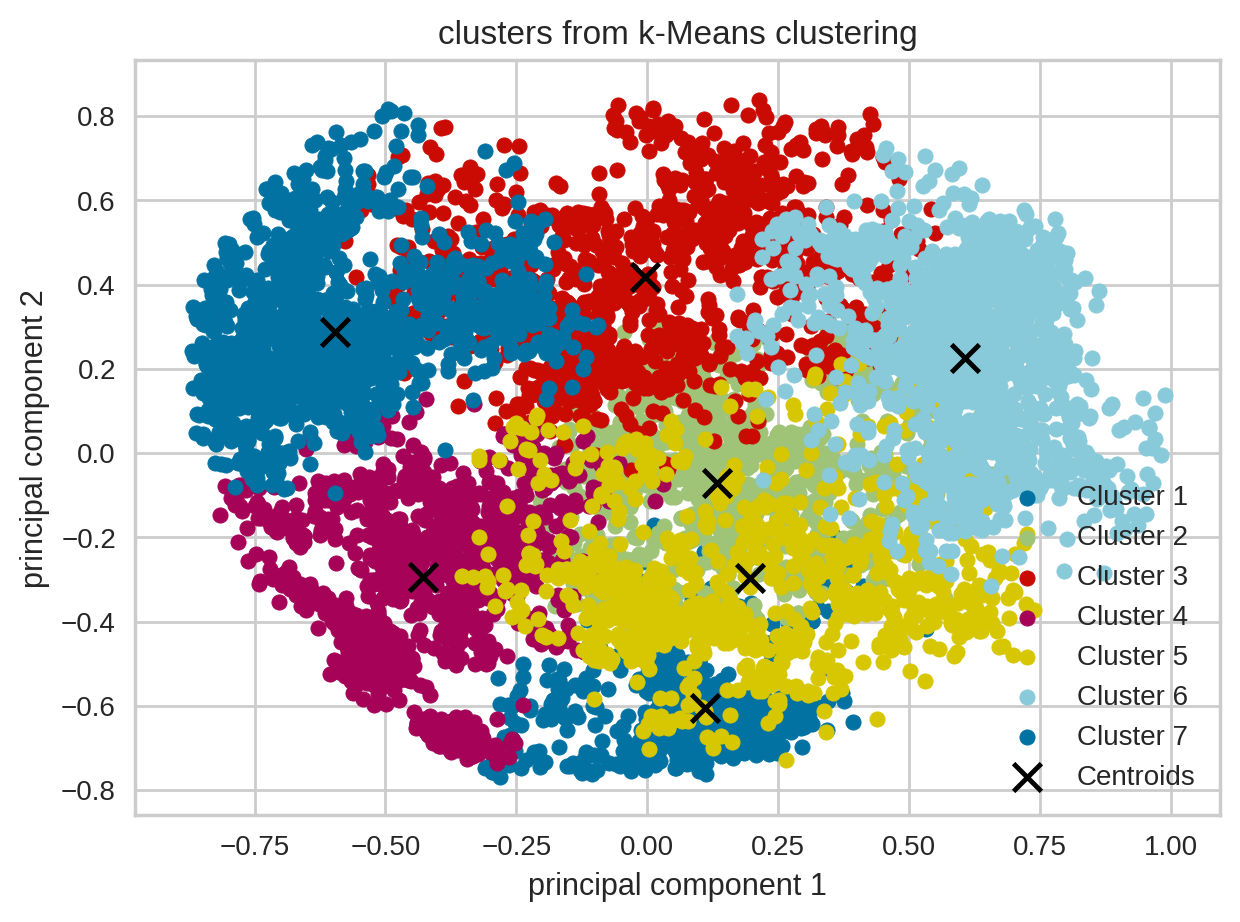
\includegraphics[width=1.0\textwidth,keepaspectratio]{images/kmeans_music.png}
    
        \column{0.5\textwidth}
        \centering
        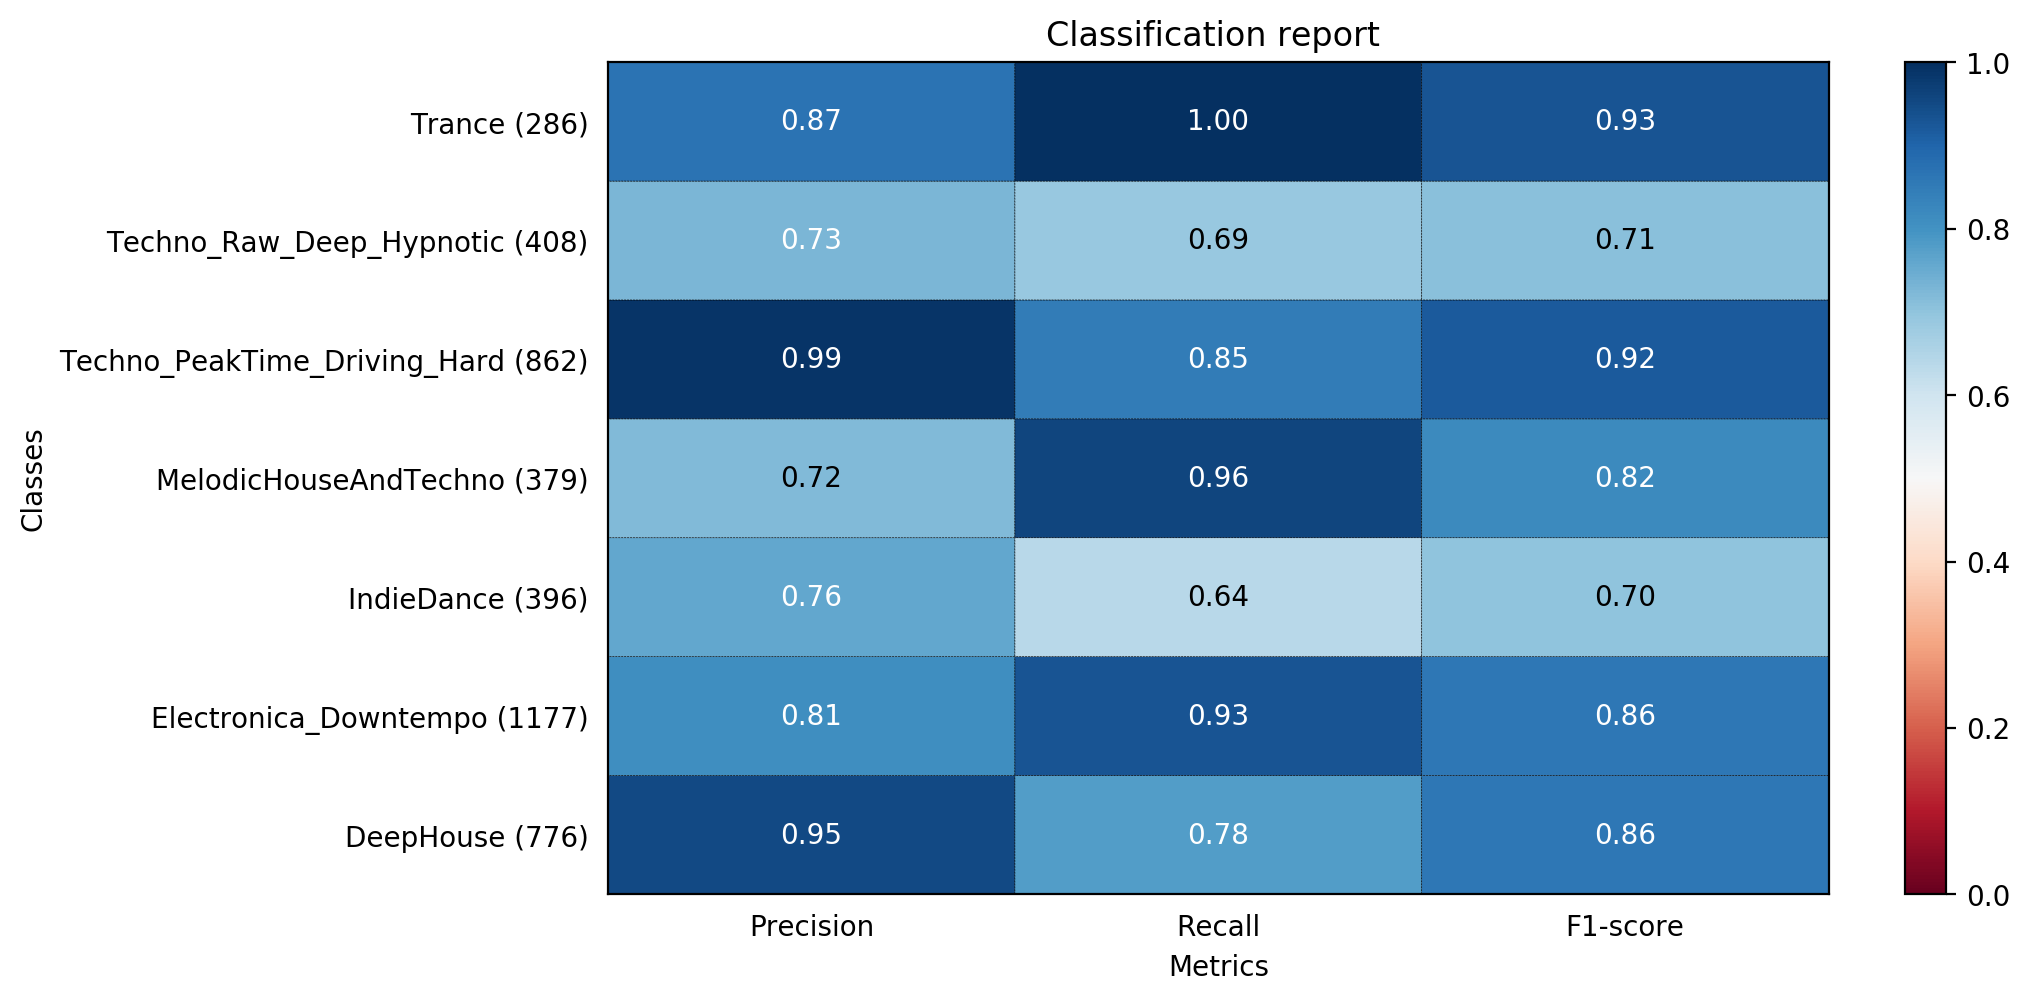
\includegraphics[width=1.0\textwidth,keepaspectratio]{images/music_plot_classif_report.png}
    \end{columns}
    
    \note{
        \begin{itemize}
            \item \textbf{17:30}
            \item the resulting model was evaluated in three different ways
            \item the first one was that the classifier, mentioned before, was trained on the music embedding space for 40 epochs, which resulted in the classification report on the right and a overall macro-averaged F1 score of 84\%
            \item the second evaluation was to apply a simple clustering algorithm, K-means, to the embedding space and to evaluate the resulting clusters\\
            -> clusters contained more of one specific label
            \item qualitative analysis done by a music expert, Mr Emanuel Oehri
        \end{itemize}
    }
\end{frame}

%%%%
\section{Conclusion and outlook}

\begin{frame}{Conclusion}
    \begin{itemize}
		\item due to the lack of time \textbf{different neural network architectures were not able to be tested}
		\item \textbf{deeper classifier on the embeddings} could improve the results of the DCASE embedding space in comparison to the challenge
		\item results of both of the \textbf{embedding spaces} showed that the space can \textbf{successfully represent and find the similarities} between audio segments
		\item \textbf{music expert} considered the results of the thesis to be a \textbf{great success}
		\item \textbf{all expected artefacts} were able to be \textbf{delivered}
		\item \textbf{project planning} could be fulfilled and was a \textbf{great help}
	\end{itemize}
	\note{
	    \begin{itemize}
	        \item \textbf{18:30}
	        \item To finalise I want to give a conclusion of the thesis and then further provide you with an outlook for future research
	    \end{itemize}
	}
\end{frame}

\begin{frame}{Outlook}
    \begin{itemize}
		\item experiment with \textbf{larger neural network architectures} to see if there is a performance gain in using them
		\item experiment with even \textbf{larger audio segments} and compare the results 
		\item implement the possibility to \textbf{generate multiple triplets from one anchor}
		\item use \textbf{continuous recordings} as dataset rather than already split samples
		\item train the embedding space using a \textbf{larger dataset with more music genres}
		\item check if the use of \textbf{transfer learning} could be used to extend the capability of the embedding space
		\item possibility of finding similarities and dissimilarities between audio segments are \textbf{beneficial for various different music tasks and applications}
	\end{itemize}
	\note{
	    \begin{itemize}
	        \item \textbf{20:00}
	    \end{itemize}
	}
\end{frame}

\begin{frame}{Questions and answers}
    \begin{center}
    {\fontsize{40}{50}\selectfont Thank You! \\[10pt] Q \& A}
    \end{center}
    \note{
    \begin{itemize}
        \item Thank you for your attention and your support throughout my thesis
        \item I'm happy to answer your questions
        \item and if you are interested, I could play some music, which was generated from walking through the embedding space after the presentation
    \end{itemize}
    }
\end{frame}

%% REFERENCES
\begin{frame}[allowframebreaks]{References}
    \begin{thebibliography}{}
        \setbeamertemplate{bibliography item}[book]
        \bibitem{DeepLearning}
        Goodfellow, Ian, Yoshua Bengio, and Aaron Courville.
        \newblock \emph{Deep Learning}.
        \newblock MIT Press, 2016.
        
        \setbeamertemplate{bibliography item}[book]
        \bibitem{MusicProcessing}
        Müller, Meinard.
        \newblock \emph{Fundamentals of Music Processing}.
        \newblock Cham: Springer International Publishing, 2015.
        
        \setbeamertemplate{bibliography item}[article]
        \bibitem{FaceNet}
        Schroff, Florian, Dmitry Kalenichenko, and James Philbin.
        \newblock \emph{FaceNet: A Unified Embedding for Face Recognition and Clustering}, 2015.
        \newblock \url{https://arxiv.org/abs/1503.03832}

        \setbeamertemplate{bibliography item}[article]
        \bibitem{Tile2Vec}
        Jean, Neal et al.
        \newblock \emph{Tile2Vec: Unsupervised representation learning for spatially distributed data}, 2018.
        \newblock \url{https://arxiv.org/abs/1805.02855}
        
        \setbeamertemplate{bibliography item}[online]
        \bibitem{DCASE}
        Dekkers, Lauwereins, Thoen et al.
        \newblock \emph{DCASE Challenge 2018 Task 5}, 2018.
        \newblock \url{http://dcase.community/challenge2018/task-monitoring-domestic-activities}
    \end{thebibliography}
\end{frame}

%% APPENDIX
\appendix

%%%% BACKUP
\begin{frame}{Related work}
	\framesubtitle{audio feature representations}
	\begin{itemize}
	    \item \textbf{sound signals} can be defined as pressure variations travelling through the air, which are often referred to as \textbf{sound waves}
		\item \textbf{raw waveform}: representations of a signal in the time-domain\\
		\begin{itemize}
		    \item x-axis: represents time
		    \item y-axis: represents amplitude
		\end{itemize}
		\item \textbf{spectrogram}: visual representation of the spectrum of frequencies of a signal as it varies with time\\
		\begin{itemize}
		    \item x-axis: represents time
		    \item y-axis: represents frequency
		    \item colours: magnitude of the frequency at a time
		\end{itemize}
	\end{itemize}
\end{frame}

\begin{frame}{Music dataset}
    \framesubtitle{Dataset used}
    \begin{table}[htbp]
        \centering
        %\caption{Music genres in the music dataset along with the number of songs}
    	\label{tab:Music-Dataset}
    	\small
        \begin{tabular}{p{.50\textwidth} | p{.10\textwidth}}
            \toprule
            \textbf{Music genres} & \textbf{\# songs} \\ 
            \midrule[1pt]
            Deep House & 30 \\
            \hline
            Electronica Downtempo & 30 \\ 
            \hline
            Indie Dance & 30 \\ 
            \hline
            Melodic House and Techno & 30 \\ 
            \hline
            Techno Peak Time Driving Hard & 30 \\ 
            \hline
            Techno Raw Deep Hypnotic & 30 \\ 
            \hline
            Trance & 30 \\
            \midrule[1pt]
            \textbf{Total} & \textbf{210} \\
            \bottomrule
        \end{tabular}
    \end{table}
\end{frame}

\begin{frame}{DCASE 2018 - task 5 dataset}
    \framesubtitle{Dataset used}
    \begin{table}[htbp]
        \centering
        %\caption[Activities performed in the dataset proposed by DCASE challenge]{Activities performed in the dataset proposed by DCASE challenge\footnotemark}
    	\label{tab:DCASE-activiies-performed}
    	\small
        \begin{tabular}{l|l|l}
            \toprule
            \textbf{Activity performed} & \textbf{\# 10s segments} & \textbf{\# sessions} \\ 
            \midrule[1pt]
            Absence (nobody present in the room) & 18860 & 42 \\
            \hline
            Cooking & 5124 & 13 \\ 
            \hline
            Dish washing & 1424 & 10 \\ 
            \hline
            Eating & 2308 & 13 \\ 
            \hline
            Other (present, but not doing any relevant activity) & 2060 & 118 \\ 
            \hline
            Social activity (visit, phone call, ...) & 4944 & 21 \\ 
            \hline
            Vacuum cleaning & 972 & 9 \\ 
            \hline
            Watching TV & 18648 & 9 \\ 
            \hline
            Working (typing, mouse clicking, ...) & 18644 & 33 \\ 
            \midrule[1pt]
            \textbf{Total} & \textbf{72984} & \textbf{268} \\
            \bottomrule
        \end{tabular}
    \end{table}
\end{frame}

\begin{frame}{Ideas and concepts}
    \framesubtitle{silhouette coefficient}
	\begin{itemize}
	    \setlength\itemsep{0em}
	    \item score is bounded between $-1$ for \textbf{incorrect clustering} and $+1$ for \textbf{highly dense clustering}
	    \item scores around $0$ indicate \textbf{overlapping clusters}
	    \item \textbf{score is higher} when clusters are \textbf{dense} and \textbf{well separated}
	    \item silhouette coefficient is defined \textbf{for each sample} and is composed of two scores:
        \begin{itemize}
            \setlength\itemsep{0em}
            \item $a$: mean distance between a sample and all other points \textbf{in the same class}
            \item $b$: mean distance between a sample and all other points \textbf{in the next nearest cluster}
        \end{itemize}
        \item silhouette coefficient $s$ for a \textbf{single sample} is then given by:
        \begin{equation}
            \centering
            s = \frac{b - a}{max(a, b)}
            \label{eq:Silhouette-Coefficient}
        \end{equation}
        \item for a \textbf{set of samples}, the silhouette coefficient is given as the \textbf{mean of the silhouette coefficient} for each sample
    \end{itemize}
\end{frame}

\begin{frame}{Ideas and concepts}
    \framesubtitle{F1 score}
	\begin{itemize}
	    \setlength\itemsep{0em}
	    \item accuracy does not work well with \textbf{highly unbalanced datasets}
	    \item \textbf{macro-averaged F1 score}, the metric has to be calculated for each label, and then the \textbf{unweighted mean} is taken
        \begin{equation}
            \centering
            \text{F1} = 2 \cdot \frac{\text{precision} \cdot  \text{recall}}{\text{precision} + \text{recall}}
        \end{equation}
        \begin{equation}
            \text{precision} = \frac{\text{TP}}{\text{TP} + \text{FP}}
        \end{equation}
        \begin{equation}
            \text{recall} = \frac{\text{TP}}{\text{TP} + \text{FN}}
        \end{equation}
        where: \\
        TP - true positive \\
        TN - true negative \\
        FP - false positive \\
        FN - false negative
    \end{itemize}
\end{frame}

\begin{frame}{Ideas and concepts}
    \framesubtitle{ResNet}
    \begin{itemize}
        \item solves the \textbf{degradation problem}, with the network depth increasing, accuracy gets saturated and then degrades rapidly
        \item \textbf{identity shortcut connection} that \textbf{skip one or more layers}
        \item double- or triple- layer skips that \textbf{contain non-linearities} (ReLU) and \textbf{batch normalization} in between
        \item residual networks are \textbf{easier to optimise} and can \textbf{gain accuracy} from considerably \textbf{increased depth}
    \end{itemize}
	\begin{columns}
        \column{0.5\textwidth}
        \centering
        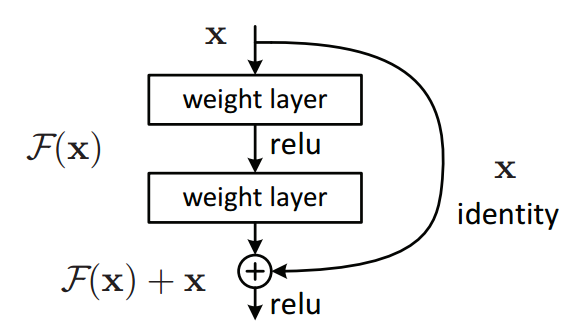
\includegraphics[width=0.8\textwidth,keepaspectratio]{images/ResNet_SkipConnections.png}
    
        \column{0.5\textwidth}
        \centering
        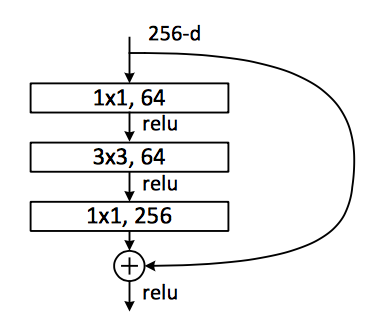
\includegraphics[width=0.6\textwidth,keepaspectratio]{images/ResNet_Stacks.png}
    \end{columns}
\end{frame}

\begin{frame}{Ideas and concepts}
    \framesubtitle{ResNet18}
	\centering
    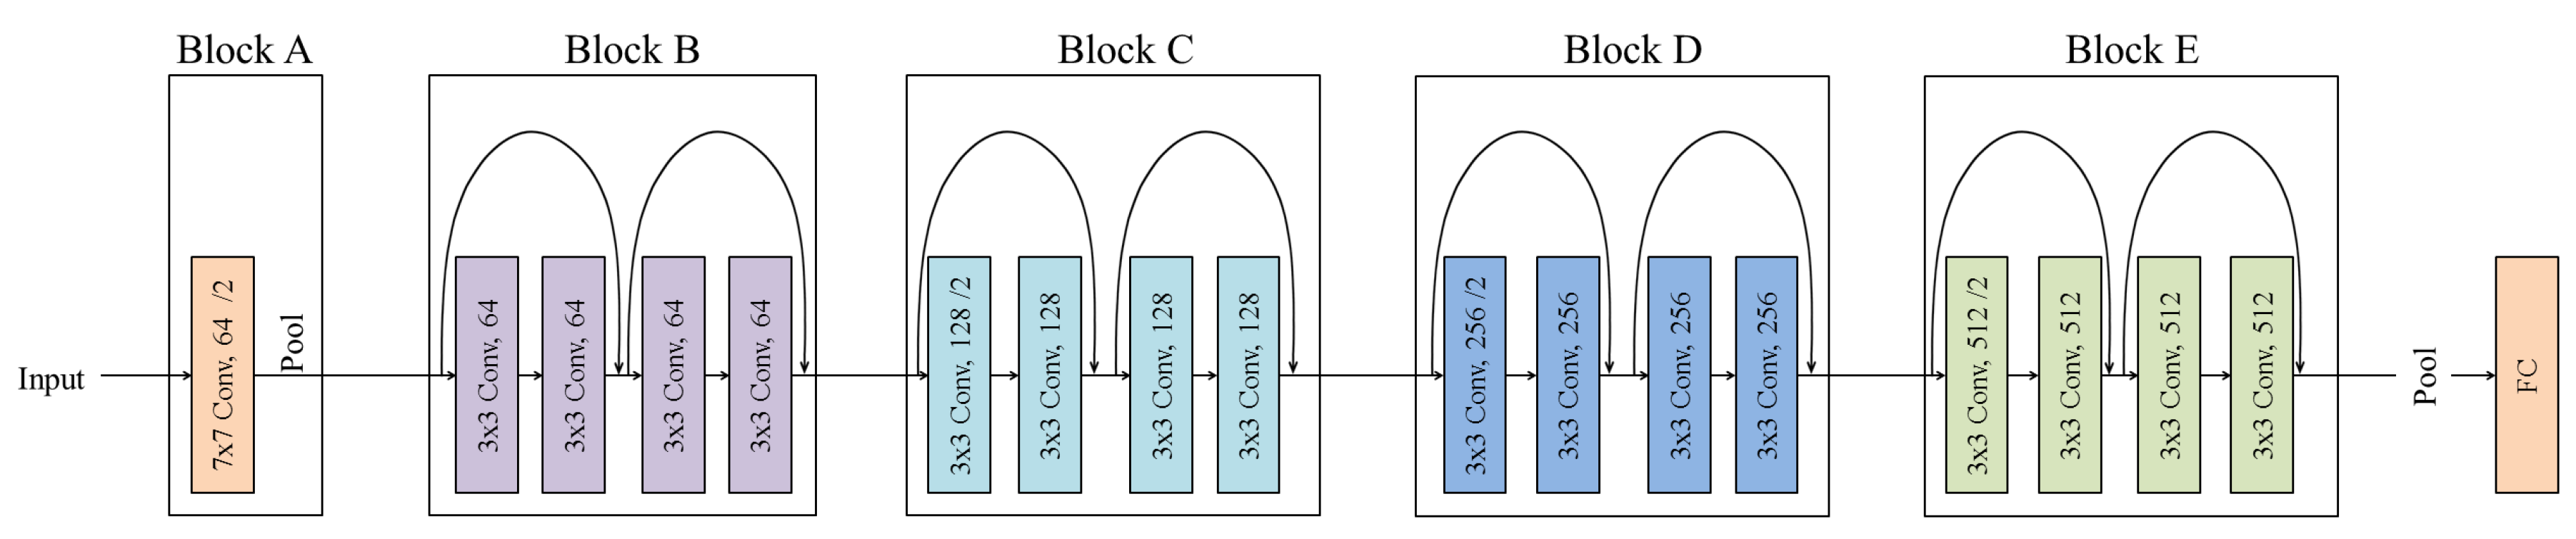
\includegraphics[width=0.95\textwidth,keepaspectratio]{images/ResNet18.png}
\end{frame}

\begin{frame}{Evaluation: DCASE 2018 - task 5 dataset}
    \framesubtitle{how will the noise detection embedding space be evaluated}

    \begin{itemize}
		\item arbitrary model trained on the {\small \texttt{development-train}} dataset and evaluated on the {\small \texttt{development-eval}} set 
		\item \textbf{simple linear logistic classifier} is trained using the embedded samples as input
		\item final evaluation using the {\small \texttt{evaluation-test}} dataset, which will be used to \textbf{compare the results to the challenge}
		\item \textbf{manual examination} of the embedding space
	\end{itemize}
    \\[10pt]
    \begin{figure}[ht]
        \centering
        \resizebox{8cm}{!}{\begin{tikzpicture}[standard/.style={inner sep=0pt,align=center,draw,text height=1.25em,text depth=0.5em},
        decoration={brace}]
        \node[text width=8cm, yshift=1cm, standard] (Trd)  {development dataset};
        \node[right=0.5em of Trd, standard, text width=4cm] (Ted)  {evaluation dataset};
        \node[fit=(Trd)(Ted), yshift=1cm, standard] (Ald)  {entire dataset from the DCASE 2018 - task 5 challenge}; 
        \node[anchor=north west, standard, text width=5.8cm, fill=yellow!30!white, yshift=-0.3cm] at (Trd.south-|Trd.west) (dev) {train};
        \node[anchor=north west, standard, text width=2cm, fill=orange!30!white, right=0.5em of dev](eval) {eval};
        \node[anchor=north west, standard, text width=4cm, fill=red!30!white, yshift=-0.3cm] at (Ted.south-|Ted.west) (Ted2) {test};
        \end{tikzpicture}}
    %\caption{Overview of the dataset split for the DCASE dataset}
    \label{fig:DCASE-split}
    \end{figure}
\end{frame}

\begin{frame}{Evaluation: music dataset}
    \framesubtitle{how will the music embedding space be evaluated}

    \begin{itemize}
		\item arbitrary model trained on the {\small \texttt{training}} dataset and evaluated on the {\small \texttt{evaluation}} set 
		\item \textbf{simple linear logistic classifier} is trained using the embedded samples as input
		\item \textbf{clustering algorithm} (K-Means) applied to the \textbf{embedding space} 
		\item \textbf{qualitative analysis} done by a music expert, Mr Emanuel Oehri
	\end{itemize}
	\\[10pt]
    \begin{figure}[ht]
        \centering
        \resizebox{8cm}{!}{\begin{tikzpicture}[standard/.style={inner sep=0pt,align=center,draw,text height=1.25em,text depth=0.5em},
        decoration={brace}]
        \node[text width=12cm, yshift=1cm, standard] (Ald)  {entire music dataset}; 
        \node[anchor=north west, standard, text width=6.8cm, fill=yellow!30!white, yshift=-0.3cm] at (Ald.south-|Ald.west) (dev) {train};
        \node[anchor=north west, standard, text width=2.4cm, fill=orange!30!white, right=0.5em of dev](eval) {eval};
        \node[anchor=north west, standard, text width=2.4cm, fill=red!30!white, right=0.5em of eval] (test) {test};
        \end{tikzpicture}}
    %\caption{Overview of the dataset split for the Music dataset}
    \label{fig:Music-split}
    \end{figure}
\end{frame}

\begin{frame}{Evaluation: Classifiers}
    \framesubtitle{how will the music embedding space be evaluated}
    
    \begin{figure}[htbp]
    \centering
    \begin{subfigure}{.5\linewidth}
      \centering
      \begin{tikzpicture}[start chain=going below, node distance=15pt,
            point/.append style={on chain, join=by {signal}},
            layer/.append style={on chain, join=by {signal}}]
            \node[point] {Input to classifier, embedded sample};
            \node[conv] {Dense layer (hidden layer 1): \\ 256 units, ReLU};
            \node[conv] {Dense layer (hidden layer 2): \\ 256 units, ReLU};
            \node[activation] {Dense output: \\ 9 units (num. of classes), softmax};
            \node[point] {Output};
        \end{tikzpicture}
      \caption{Dense classifier}
      \label{fig:dense-classifier}
    \end{subfigure}%
    \begin{subfigure}{.5\linewidth}
      \centering
      \begin{tikzpicture}[start chain=going below, node distance=15pt,
            point/.append style={on chain, join=by {signal}},
            layer/.append style={on chain, join=by {signal}}]
            \node[point] {Input to classifier, embedded sample};
            \node[activation] {Dense output: \\ 9 units (num. of classes), softmax};
            \node[point] {Output};
        \end{tikzpicture}
      \caption{Linear logistic classifier}
      \label{fig:logistic-classifier}
    \end{subfigure}
    \caption{Visualisation of the different classifier architectures}
    \label{fig:Classifier-DCASE-Visualisation}
    \end{figure}
\end{frame}

\begin{frame}{Results: music dataset}
    \framesubtitle{final model trained on the music dataset}
    
    \centering
    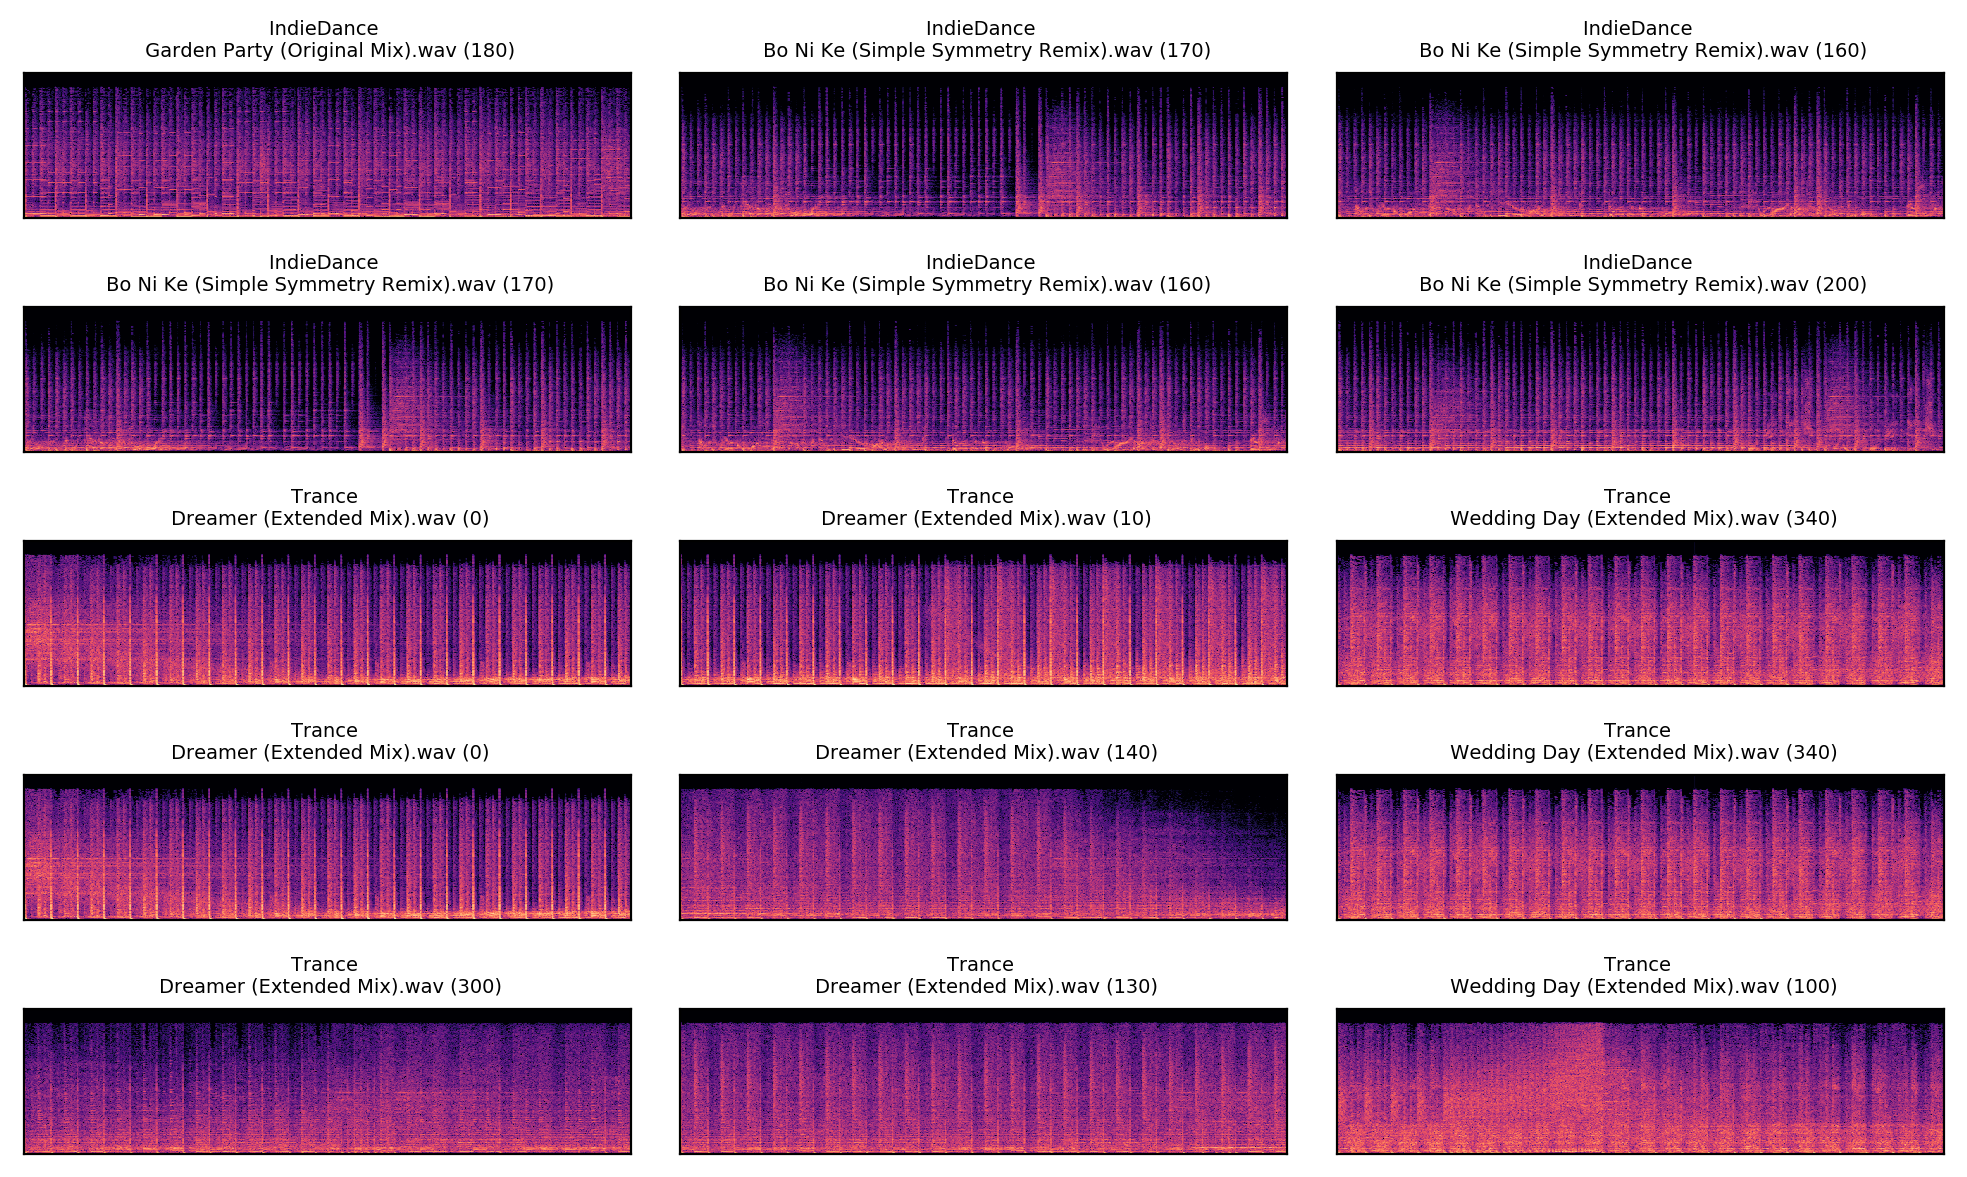
\includegraphics[width=0.7\textwidth,keepaspectratio]{images/Walk_through_music_space.png}
    
    \note{
        \begin{itemize}
            \item Play walk through the space
        \end{itemize}
    }
\end{frame}

%%
\end{document}